\section{Algorithmen}

Verteilte Systeme stehen vor einer Vielzahl von Herausforderungen und Problemklassen, die gelöst werden müssen, um ein effizientes und zuverlässiges Funktionieren zu gewährleisten. Hier sind einige der wichtigsten Problemklassen in verteilten Systemen, die durch Algorithmen und Protokolle gelöst oder zumindest approximiert werden können:
\begin{itemize}
\item Konsensprobleme: Wie zuvor diskutiert, müssen verteilte Systeme oft eine Einigung über einen bestimmten Wert oder Zustand erreichen. Algorithmen wie Paxos und Raft sind Lösungen für das Konsensproblem.

\item Koordinationsprobleme: Verteilte Systeme müssen oft die Ausführung von Operationen koordinieren. Dies kann so einfach sein wie das Sperren von Ressourcen während der Bearbeitung oder so komplex wie die Durchführung von Transaktionen, die mehrere Knoten betreffen. Algorithmen und Protokolle wie Two-Phase Commit (2PC) und Three-Phase Commit (3PC) bieten Lösungen für solche Koordinationsprobleme.

\item Replikations- und Konsistenzprobleme: Verteilte Systeme replizieren oft Daten auf mehrere Knoten, um die Ausfallsicherheit zu verbessern und die Zugriffszeiten zu verkürzen. Dies wirft jedoch Probleme der Konsistenz auf: Wie kann sichergestellt werden, dass alle Kopien eines Datenobjekts immer den gleichen Zustand haben? Es gibt eine Vielzahl von Konsistenzmodellen und Replikationsstrategien (wie z.B. quorumbasierte oder eventual consistency Ansätze), die dazu beitragen, diese Herausforderungen zu bewältigen.

\item Fehlertoleranz- und Wiederherstellungsprobleme: Verteilte Systeme müssen robust gegenüber Ausfällen einzelner Knoten oder Netzwerkteile sein und in der Lage sein, sich von solchen Ausfällen zu erholen. Techniken wie Redundanz, Checkpointing und Protokollierung, sowie Algorithmen für die Fehlererkennung und Wiederherstellung spielen hier eine wichtige Rolle.

\item Lastverteilungs- und Ressourcenverwaltungsprobleme: Verteilte Systeme müssen die Ressourcen, einschließlich Rechenleistung, Speicher und Netzwerkbandbreite, effizient verwalten und verteilen. Dies kann durch Lastverteilungsalgorithmen und Ressourcenverwaltungssysteme erreicht werden.
\end{itemize}

Insgesamt ist die effektive Bewältigung dieser und anderer Problemklassen in verteilten Systemen eine komplexe Aufgabe, die eine sorgfältige Planung, Design und Implementierung erfordert. Trotzdem bieten die Algorithmen und Techniken, die in der Forschung und Praxis der verteilten Systeme entwickelt wurden, leistungsfähige Werkzeuge zur Lösung oder zumindest Approximation dieser Probleme.

Dieses Kapitel versucht den Fokus weniger auf die Algorithmik zu legen und gibt Einblicke in die grundsätzliche Konstruktion und die damit verbundenen Eigenschaften.

\subsection{Paralleles Rechnen}

Paralleles Rechnen ist eine Form der Berechnung, bei der viele Berechnungen gleichzeitig ausgeführt werden, indem ein Problem in konkurrierende Unteraufgaben aufgeteilt wird, die gleichzeitig ausgeführt werden. In verteilten Systemen, wie z.B. in einem Cluster von Computern oder einem Netzwerk von Knoten, kann die parallele Ausführung von Algorithmen die Gesamtleistung der Systeme erheblich verbessern.


Es gibt viele Algorithmen, die sich gut für eine hohe Parallelisierung eignen, insbesondere solche, die \enquote{embarrassingly parallel} sind, d.h. sie lassen sich leicht in unabhängige Unteraufgaben aufteilen, die gleichzeitig ausgeführt werden können. Hier sind einige Beispiele:

\begin{itemize}
\item Matrixoperationen: Matrixmultiplikation, Matrixtransposition und andere Matrixoperationen können in viele unabhängige Aufgaben aufgeteilt werden, die jeweils auf verschiedenen Prozessoren ausgeführt werden können.
\item Sortieralgorithmen: Einige Sortieralgorithmen, wie der Mergesort, lassen sich gut parallelisieren. Der Array kann in mehrere Segmente aufgeteilt werden, die unabhängig voneinander sortiert und anschließend zusammengeführt werden können.
\item Grafikverarbeitung: Viele Grafik- und Bildverarbeitungsalgorithmen sind stark parallelisierbar. Dies umfasst Operationen wie das Rendering von 3D-Grafiken, die Anwendung von Filtern auf Bilder oder die Durchführung von Kanten- oder Feature-Erkennungen in Bildern.
\item Molekulardynamiksimulationen: In der Physik und Chemie können große Simulationen, wie z. B. Molekulardynamiksimulationen, stark parallelisiert werden, indem das System in mehrere Teile aufgeteilt und die Interaktionen innerhalb jedes Teils unabhängig berechnet werden.
\item Monte-Carlo-Simulationen: Diese Art von Simulationen, die auf einer großen Anzahl von zufälligen Proben beruhen, sind oft stark parallelisierbar, da jede Probe unabhängig von den anderen ist.
\item Maschinelles Lernen: Viele Algorithmen im Bereich des maschinellen Lernens, insbesondere im Deep Learning, können stark parallelisiert werden. Dies gilt insbesondere für das Training von neuronalen Netzen, bei dem die Gewichtsaktualisierungen oft unabhängig für viele Neuronen gleichzeitig berechnet werden können.
\end{itemize}

Es gibt unterschiedliche Programmiermodelle und Frameworks, die das verteilte Rechnen in besonderer Art unterstützten. 
MapReduce (Hadoop) und Resilient Distributed Datasets (Spark) sind beides Frameworks zur Verarbeitung großer Datenmengen auf verteilten Systemen, aber sie verwenden unterschiedliche Ansätze und sollen in diesem Skript exemplarisch besprochen werden.

MapReduce ist ein Programmiermodell, das von Google entwickelt und in Apache Hadoop implementiert wurde. Es ist speziell für die Verarbeitung großer Datenmengen in einem verteilten Umfeld ausgelegt. MapReduce besteht aus zwei Hauptphasen: Map und Reduce.
\begin{itemize}
\item Map: In der Map-Phase werden die Eingabedaten in Schlüssel-Wert-Paare aufgeteilt und dann unabhängig voneinander verarbeitet. Jeder Map-Arbeiter arbeitet auf einem lokalen Datensatz und erzeugt eine Liste von Zwischenschlüssel-Wert-Paaren.
\item Reduce: In der Reduce-Phase sammelt der Master-Arbeiter die Zwischenschlüssel-Wert-Paare von den Map-Arbeitern, sortiert sie nach Schlüssel und leitet sie an die Reduce-Arbeiter weiter. Jeder Reduce-Arbeiter verarbeitet dann alle Werte, die zu einem bestimmten Schlüssel gehören, und erzeugt einen endgültigen Satz von Schlüssel-Wert-Paaren. 
\end{itemize}
Apache Hadoop ist eine weit verbreitete Open-Source-Implementierung des MapReduce-Modells. 

Resilient Distributed Datasets (RDDs) sind eine zentrale Komponente des Apache Spark-Frameworks. Im Gegensatz zu MapReduce, das auf die Ausführung einzelner Jobs ausgelegt ist, wurde Spark entwickelt, um Workflows mit mehreren Jobs und interaktive Abfragen zu unterstützen.

Ein RDD ist eine Sammlung von Elementen, die über die Knoten eines Clusters verteilt sind und parallel verarbeitet werden können. RDDs sind unveränderlich und können durch Transformationen wie map, filter und reduce erzeugt werden. Wenn Daten einmal in einen RDD geladen wurden, können sie im Arbeitsspeicher gehalten und für mehrere Operationen wiederverwendet werden, was zu erheblichen Leistungsverbesserungen führen kann.

Apache Spark unterstützt auch Operationen, die über Map und Reduce hinausgehen, wie z.B. Sortieren, Gruppieren und Joinen von Daten. Darüber hinaus bietet es Unterstützung für maschinelles Lernen, Graphverarbeitung und Streamverarbeitung durch zusätzliche Bibliotheken.


Aber es weiter wichtig zu verstehen, dass nicht alle Algorithmen gut für die Parallelisierung geeignet sind. Einige Probleme, wie das Suchen in einer sortierten Liste, können effizient parallelisiert werden, während andere, wie das Berechnen des größten gemeinsamen Teilers (ggT), nicht so offensichtlich parallelisierbar sind.

Um die Herausforderungen deutlich zu machen, soll an dem Fallbeispiel ggt ein beispielhaftes Vorgehen besprochen werden. Der ggt ist ein sehr klassisches Beispiel für diese Klasse von Herausforderungen. 

Der ggT von zwei Zahlen ist die größte Zahl, die beide Zahlen ohne Rest teilt. Ein weit verbreiteter Algorithmus zur Berechnung des ggT ist der euklidische Algorithmus, der auf einer Reihe von Divisionen basiert. Dieser Algorithmus ist schwer zu parallelisieren, da jede Division auf dem Ergebnis der vorherigen basiert. Es gibt jedoch einige Ansätze zur Parallelisierung.

Angenommen, wir haben eine Liste von Paaren von Zahlen und wir wollen den ggT für jedes Paar berechnen. In einem sequenziellen System würde man durch die Liste gehen und für jedes Paar den ggT berechnen. In einem verteilten System könnte man jedoch die Berechnung des ggT für jedes Paar auf einem separaten Knoten ausführen. Auf diese Weise würden alle ggT-Berechnungen gleichzeitig ausgeführt werden.

Folgendermaßen könnte das in Pseudocode dargestellt werden:

\begin{lstlisting}[caption={ggT},captionpos=b,label={lst:ggt}]
function berechne_ggt_liste(liste_von_paaren):
    ggt_liste = leere Liste
    fuer jedes Paar in liste_von_paaren:
        sende Paar an einen freien Knoten zur Berechnung
    fuer jedes Paar in liste_von_paaren:
        empfange ggt von Knoten und fuege es zu ggt_liste hinzu
    return ggt_liste
\end{lstlisting}

In diesem Fall ist die Parallelisierung auf der Ebene der Paare und nicht auf der Ebene der einzelnen ggT-Berechnung. Es gibt also eine Granularität bei der Parallelisierung: Manchmal kann man die einzelnen Schritte eines Algorithmus parallelisieren, und manchmal kann man verschiedene Instanzen des gesamten Algorithmus parallelisieren.

Angenommen, wir haben eine Liste von drei Paaren von Zahlen: (48, 18), (49, 21) und (36, 15). Wir wollen den ggT für jedes Paar berechnen.

In diesem Beispiel würde der Master-Knoten das Paar (48, 18) an den ersten Knoten senden, das Paar (49, 21) an den zweiten Knoten und das Paar (36, 15) an den dritten Knoten. Jeder Knoten würde dann den ggT für sein Paar berechnen und das Ergebnis an den Master-Knoten senden.

Die ggT-Berechnung könnte folgendermaßen aussehen:
\begin{itemize}
\item Knoten 1 berechnet den ggT von 48 und 18. Der Euklidische Algorithmus gibt 6 als Ergebnis.
\item Knoten 2 berechnet den ggT von 49 und 21. Der Euklidische Algorithmus gibt 7 als Ergebnis.
\item Knoten 3 berechnet den ggT von 36 und 15. Der Euklidische Algorithmus gibt 3 als Ergebnis.
\end{itemize}
Der Master-Knoten würde dann die Ergebnisse empfangen und eine Liste der ggT erstellen: [6, 7, 3].

In diesem Beispiel erfolgt die Parallelisierung auf der Ebene der Paare und nicht auf der Ebene der einzelnen ggT-Berechnung. Es ist wichtig zu beachten, dass die Kommunikation zwischen den Knoten auch Zeit kostet, und diese Zeit sollte bei der Beurteilung der Gesamtleistung des verteilten Systems berücksichtigt werden.

Die Berechnung des größten gemeinsamen Teilers (ggT) für eine große Menge von Zahlpaaren könnte auch mit MapReduce in Hadoop umgesetzt werden. Da die Map- und Reduce-Schritte würden allerdings in diesem Fall nicht auf die traditionelle Weise verwendet, da die ggT-Berechnung nicht leicht in unabhängige Map- und Reduce-Operationen zerlegt werden kann.

Stattdessen wirt der Map-Schritt verwendet, um die ggT-Berechnung für jedes Paar durchzuführen, und den Reduce-Schritt, um die Ergebnisse zu sammeln. Hier ist ein Pseudocode, der zeigt, wie das gemacht werden könnte:

\begin{lstlisting}[caption={Map- und Reduce},captionpos=b,label={lst:map_e}]
public class GgtBerechnung {

  public static class Map extends Mapper<LongWritable, Text, Text, IntWritable> {
    public void map(LongWritable key, Text value, Context context) throws IOException, InterruptedException {
      String[] zahlenpaar = value.toString().split(",");
      int a = Integer.parseInt(zahlenpaar[0]);
      int b = Integer.parseInt(zahlenpaar[1]);
      
      // Berechnen Sie den ggT
      while (b != 0) {
        int temp = b;
        b = a % b;
        a = temp;
      }
      
      // Schreiben Sie das Ergebnis in den Kontext
      context.write(new Text("ggT"), new IntWritable(a));
    }
  }

  public static class Reduce extends Reducer<Text, IntWritable, Text, IntWritable> {
    public void reduce(Text key, Iterable<IntWritable> values, Context context) throws IOException, InterruptedException {
      // Schreiben Sie jedes Ergebnis in den Kontext
      for (IntWritable val : values) {
        context.write(key, val);
      }
    }
  }
}
\end{lstlisting}

In diesem Beispiel würde die Eingabe als Textformat erwartet, mit jedem Paar von Zahlen durch ein Komma getrennt und jedes Paar auf einer eigenen Zeile. Der Map-Schritt würde den ggT für jedes Paar berechnen, und der Reduce-Schritt würde die Ergebnisse sammeln und ausgeben. 

Es ist wichtig zu beachten, dass dieser Ansatz nur dann sinnvoll ist, wenn die Anzahl der Paare groß genug ist, um die Overheadkosten der Verwendung eines verteilten Systems wie Hadoop zu rechtfertigen.

Auch Apache Spark eignet sich eher für datenintensive Aufgaben wie die Verarbeitung großer Mengen von Textdaten, Bildern oder Netzwerklogs. Die Berechnung des größten gemeinsamen Teilers (ggT) ist eine rechenintensive Aufgabe, die im Allgemeinen nicht gut auf ein verteiltes Datensystem wie Spark passt, insbesondere da der Euklidische Algorithmus für die ggT-Berechnung schwer zu parallelisieren ist.

Allerdings könnten wir, wenn wir eine große Anzahl von Paaren von Zahlen hätten und den ggT für jedes Paar berechnen wollten, diese Berechnung auf einem Spark-Cluster durchführen. Hier ist ein einfacher Pseudocode, der zeigt, wie das gemacht werden könnte:

\begin{lstlisting}[caption={RDD Spark},captionpos=b,label={lst:spark}]

# Definieren Sie eine Funktion zur Berechnung des ggT
def berechne_ggt(paar):
    a, b = paar
    while b != 0:
        a, b = b, a % b
    return a

# Erstellen Sie ein RDD aus den Eingabepaaren
paare = spark.parallelize([(48, 18), (49, 21), (36, 15)])

# Berechnen Sie den ggT fuer jedes Paar
ggts = paare.map(berechne_ggt)

# Sammeln Sie die Ergebnisse
ergebnisse = ggts.collect()


\end{lstlisting}

Es ist zu beachten, dass die Kommunikation zwischen den Knoten in einem verteilten System auch Zeit in Anspruch nimmt. Wenn die ggT-Berechnung sehr schnell ist, kann es sein, dass die Kommunikationszeit den größten Teil der gesamten Berechnungszeit ausmacht. In solchen Fällen könnte es effizienter sein, mehrere ggT-Berechnungen auf einem Knoten auszuführen, bevor die Ergebnisse gesendet werden. Dies wird als Bündelung oder Batch-Verarbeitung bezeichnet.

Parallelisierung in verteilten Systemen ist ein komplexes Thema, das eine sorgfältige Abwägung von Faktoren wie der Granularität der Parallelisierung, der Kommunikationszeit zwischen den Knoten und der Lastverteilung erfordert. Es ist jedoch ein mächtiges Werkzeug, das in der Lage ist, die Berechnungszeit erheblich zu reduzieren und die Leistung von Algorithmen in großen Systemen zu steigern.

Es ist auch wichtig zu beachten, dass Fehlermanagement und Wiederherstellungsstrategien in verteilten Systemen eine entscheidende Rolle spielen. Knotenausfälle, Netzwerkprobleme und andere Störungen können die Berechnung beeinträchtigen. Daher müssen robuste Mechanismen implementiert werden, um solche Probleme zu erkennen und zu beheben.

Dazu gehört die Überwachung der Knoten, um sicherzustellen, dass sie funktionieren und ihre Aufgaben erfolgreich abschließen. Bei einem Ausfall kann der Master-Knoten die Aufgabe erneut an einen anderen Knoten senden. Außerdem können Checkpoints verwendet werden, um den Fortschritt der Berechnung zu speichern und bei einem Ausfall von diesem Punkt aus fortzufahren.

Im Folgenden werden auch die Punkte besprochen, die zur Konsensbildung und Fehlertoleranz in zentralisierten oder dezentralisierten Ansätzen umgesetzt werden können.

Wie auch immer, die Wahl des richtigen Ansatzes zur Parallelisierung kann stark von der Art des Problems, den verfügbaren Ressourcen und der spezifischen Umgebung abhängen. Die Entwicklung und Optimierung paralleler Algorithmen in verteilten Systemen erfordert ein tiefes Verständnis der Algorithmen, der Systemarchitektur und der zugrunde liegenden Technologien.

Letztlich ist das Ziel der Parallelisierung in verteilten Systemen, die Gesamtleistung zu steigern und die Berechnungszeit zu reduzieren. Dies kann erreicht werden, indem Aufgaben aufgeteilt und gleichzeitig auf mehreren Knoten ausgeführt werden. Obwohl dies eine Herausforderung sein kann, bietet es auch eine großartige Gelegenheit, die Leistungsfähigkeit moderner Computer und Netzwerke voll auszuschöpfen.


\subsection{Zentralisierte vs. dezentralisierte Algorithmen}

Verteilte Systeme sind Netzwerke von unabhängigen Computern, die unter anderem so konfiguriert sind, dass sie als ein einziges System arbeiten. Die Hauptvorteile verteilter Systeme sind Skalierbarkeit, Fehlertoleranz und Ressourcenfreigabe.

Verteilte Systeme setzen Algorithmen ein, um die Koordination zwischen den Knoten zu gewährleisten. Einige der Hauptkategorien dieser Algorithmen sind Kommunikationsprotokolle, Synchronisationsalgorithmen, Fehlererkennung und -behandlung, Scheduling, Datenkonsistenz und Replikationsstrategien.

In Bezug auf die Struktur der Verteilung können wir zentralisierte und dezentralisierte Algorithmen unterscheiden:

\begin{itemize}
\item Zentralisierte Algorithmen setzen auf einen oder wenige zentrale Knoten, die die meisten oder alle Entscheidungen treffen. Ein typisches Beispiel wäre ein Client-Server-System, in dem der Server die zentrale Kontrollinstanz ist. Ein zentrales System kann einfacher zu entwerfen und zu verwalten sein. Es kann auch einfacher sein, in Bezug auf Sicherheit und Datenkonsistenz. Allerdings haben zentralisierte Systeme eine höhere Anfälligkeit für Ausfälle und können Engpässe aufweisen, da alle Anfragen durch die zentrale Einheit gehen müssen.

\item Dezentralisierte Algorithmen dagegen verteilen die Verantwortung auf alle Knoten im Netzwerk. Ein typisches Beispiel wäre ein Peer-to-Peer-Netzwerk, bei dem alle Knoten gleichberechtigt sind und Ressourcen teilen. Dezentralisierte Systeme sind in der Regel robuster und skalierbarer, da sie nicht von einem zentralen Knoten abhängen. Allerdings sind sie oft komplexer zu entwerfen und zu verwalten, und es kann schwieriger sein, Datenkonsistenz und Sicherheit zu gewährleisten.
\end{itemize}

Bei der Entscheidung zwischen zentralisierten und dezentralisierten Algorithmen muss sorgfältig geprüft werden:
\begin{itemize}
\item Leistung: Zentralisierte Algorithmen können schneller sein, da sie weniger Koordination erfordern. Aber wenn das System skaliert, können Engpässe entstehen. Dezentralisierte Algorithmen können besser skalieren, aber sie können aufgrund der größeren Anzahl von Nachrichten, die zwischen den Knoten ausgetauscht werden, mehr Netzwerkbandbreite erfordern.
\item Zuverlässigkeit: Zentralisierte Algorithmen sind anfälliger für Ausfälle, da der Ausfall des zentralen Knotens das gesamte System lahmlegen kann. Dezentralisierte Algorithmen sind in der Regel widerstandsfähiger gegen Ausfälle, da es keine einzelne Fehlerstelle gibt.
\item Konsistenz: Zentralisierte Algorithmen können eine stärkere Konsistenz gewährleisten, da alle Änderungen durch den zentralen Knoten koordiniert werden. Dezentralisierte Algorithmen können eine schwächere Konsistenz haben, da Änderungen unabhängig voneinander vorgenommen werden können und es Zeit braucht, bis sie sich im gesamten System verbreiten.
\item Sicherheit: Zentralisierte Algorithmen können einfacher zu sichern sein, da alle Zugriffe durch den zentralen Knoten kontrolliert werden können. Bei dezentralisierten Algorithmen ist es schwieriger, den Zugriff zu kontrollieren und bösartige Knoten zu erkennen.
\end{itemize}
Die spezifischen Algorithmen, die in einem verteilten System verwendet werden, wie One-to-Many-Kommunikation, Baumstrukturen, Flooding oder Gossip, hängen ebenfalls von den Anforderungen des Systems ab. Jede dieser Methoden hat ihre eigenen Vor- und Nachteile und ist für bestimmte Arten von Anwendungen besser geeignet.

Zum Beispiel kann die One-to-Many-Kommunikation nützlich sein, wenn ein Knoten häufig Updates an eine Gruppe von anderen Knoten senden muss. Baumstrukturen können hilfreich sein, wenn die Daten in einer hierarchischen Struktur organisiert sind oder wenn effiziente Such- und Sortieroperationen erforderlich sind. Flooding kann nützlich sein, um sicherzustellen, dass eine Nachricht alle Knoten erreicht, aber es kann zu einer übermäßigen Netzwerkbelastung führen. Gossip-Algorithmen können effizient sein, um Informationen schnell zu verbreiten, aber sie können zu einer schwächeren Konsistenz führen.


\subsection{Konsens}

Viele der Institutionen, auf die wir als moderne Gesellschaft angewiesen sind - Krankenhäuser, Banken, Börsen und Flughäfen - benötigen hochzuverlässige und stets verfügbare Computersysteme, um funktionieren zu können. Leider sind einzelne Maschinen dieser Herausforderung nicht gewachsen. Sie sind anfällig für Ausfälle und Stillstandzeiten und bedürfen regelmäßiger Wartung. Die Lösung besteht natürlich darin, mehrere Maschinen für dieselbe Aufgabe einzusetzen. Doch wie bringen wir sie dazu? Dies ist keine einfache Aufgabe. Die Netzwerkverbindungen zwischen den Maschinen sind nicht zuverlässig, die Maschinen selbst können ausfallen und wir möchten nicht, dass Menschen Dinge um drei Uhr morgens an einem Sonntag reparieren müssen. Konsens ist ein grundlegender Bestandteil beim Aufbau replizierter Systeme und um diese Maschinen zusammenarbeiten zu lassen. Die Idee, sie zur Zusammenarbeit zu bringen, besteht darin, dass alle dieselben Daten oder Befehle in ihren Protokollen speichern. Dies erhöht die Gesamtzuverlässigkeit des Systems, denn wenn eine Maschine ausfällt, kann eine andere Maschine ihre Arbeit übernehmen.

Konsensalgorithmen spielen eine entscheidende Rolle in verteilten Systemen, indem sie sicherstellen, dass alle Knoten, trotz möglicher Fehlfunktionen einiger Knoten oder Netzwerkprobleme, zu einer gemeinsamen Sicht auf den Systemzustand gelangen. Der Konsens ist ein fundamentales Problem in der verteilten Systemforschung und es gibt eine Vielzahl von Algorithmen, die entwickelt wurden, um dieses Problem zu lösen.

Im Wesentlichen besteht das Konsensproblem darin, dass eine Gruppe von Prozessen oder Knoten, die möglicherweise fehlerhaft sind oder in einem fehlerhaften Netzwerk operieren, sich auf einen gemeinsamen Wert einigen muss. Das Konsensproblem wird noch komplexer, wenn man bedenkt, dass Knoten gleichzeitig abstimmen und unterschiedliche Informationen haben können. Ein zuverlässiger Konsensalgorithmus muss in der Lage sein, trotz dieser Herausforderungen einen einheitlichen Wert zu ermitteln.

Bevor das geschieht, soll ein Anwendungsbeispiel besprochen werden, was die grundsätzliche Herangehensweise bespricht.  In diesem Anwendungsbeispiel handelt es sich um ein verteiltes System von zwei Ampeln, das den Verkehr an einer Baustelle reguliert. Dies ist ein gutes Anwendungsbeispiel für einen verteilten Algorithmus, da jede Ampel autonom arbeitet und gleichzeitig mit der anderen koordiniert werden muss, um einen sicheren Verkehrsfluss zu gewährleisten.

Ein geeigneter Algorithmus für diese Situation wäre ein einfacher Konsensalgorithmus. In diesem Szenario könnte der \enquote{Zustand} jeder Ampel (rot oder grün) als eine Art \enquote{Vorschlag} für den nächsten Zustand des Systems betrachtet werden. Jede Ampel könnte dann einen Konsensalgorithmus verwenden, um sicherzustellen, dass beide Ampeln sich auf den gleichen nächsten Zustand einigen (d.h., eine Ampel ist rot und die andere ist grün).

Hier ist, wie der Algorithmus funktionieren könnte:
\begin{itemize}
\item Jede Ampel beginnt in einem sicheren Zustand (rot).
\item  Wenn eine Ampel auf grün umschalten möchte, sendet sie eine Nachricht an die andere Ampel, um sie über ihre Absicht zu informieren.
\item Wenn die andere Ampel die Nachricht erhält, prüft sie ihren eigenen Zustand. Wenn sie grün ist, bleibt sie grün und sendet eine Ablehnungsnachricht zurück. Wenn sie rot ist, sendet sie eine Bestätigungsnachricht zurück.
\item  Die ursprüngliche Ampel kann auf grün umschalten, wenn sie eine Bestätigungsnachricht erhält. Wenn sie eine Ablehnungsnachricht erhält, bleibt sie rot.
\end{itemize}
In diesem Szenario wäre der Beobachter, der den korrekten Zustand der Ampeln ermittelt, derjenige, der den aktuellen Zustand jeder Ampel und die von jeder Ampel gesendeten Nachrichten berücksichtigt.

Dieser Algorithmus stellt sicher, dass zu keinem Zeitpunkt beide Ampeln gleichzeitig grün sind und dass jede Ampel autonom auf rot umschalten kann, wenn sie dies für notwendig hält. Es ist wichtig zu beachten, dass in der Realität die Ampelsteuerung aufgrund von Faktoren wie Fußgängerüberwegen, mehreren Fahrspuren und so weiter komplexer sein kann, aber dieses einfache Modell dient als eine gute Einführung in die Art und Weise, wie verteilte Algorithmen zur Koordination autonomer Systeme verwendet werden können.
In diesem Beispiel allerdings verhalten sich alle Teilnehmer korrekt und fehlerfrei.

Die grundlegenden Anforderungen für einen Konsensalgorithmus sind:
\begin{itemize}
\item Einigkeit: Alle nicht fehlerhaften Knoten müssen sich auf denselben Wert einigen.
\item Integrität: Ein Knoten entscheidet sich höchstens einmal für einen Wert, und wenn es sich für einen Wert entscheidet, muss dieser Wert von einem der Knoten vorgeschlagen worden sein.
\item Terminierung: Alle nicht fehlerhaften Knoten müssen schließlich eine Entscheidung treffen.
\item Validität: Wenn alle Knoten denselben anfänglichen Wert haben, dann müssen sie sich auf diesen Wert einigen.
\end{itemize}
Die bekanntesten Konsensalgorithmen sind Paxos, Raft und Zab (ZooKeeper Atomic Broadcast). Paxos, von Leslie Lamport entworfen, ist bekannt für seine Korrektheit, aber auch für seine Komplexität. Raft wurde entwickelt, um einen einfacheren, leichter zu verstehenden Konsensalgorithmus zu bieten, der dennoch die gleiche Leistung und Korrektheit wie Paxos bietet. Zab ist ein Konsensprotokoll, das speziell für ZooKeeper, ein Dienst für verteilte Koordination von Apache, entwickelt wurde.

Diese Algorithmen haben jeweils ihre Stärken und Schwächen und können in unterschiedlichen Szenarien und für verschiedene Anforderungen geeignet sein. Die Wahl des richtigen Konsensalgorithmus für ein bestimmtes verteiltes System erfordert daher eine sorgfältige Überlegung verschiedener Faktoren, einschließlich der Systemgröße, der Häufigkeit von Netzwerkfehlern, der Anforderungen an die Datenkonsistenz und der Leistungsanforderungen. Doch bevor Paxos, Raft und Co. im Detail diskutiert werden sind noch ein paar Vorarbeiten mit Algorithmen zu erledigen, die notwendige Wahlen realisieren oder Ordnung etablieren.

\subsubsection{Follow the Leader}
\enquote{Follow the Leader} ist eine Strategie, die in vielen verteilten Konsensprotokollen wie Raft und ZAB verwendet wird. Bei dieser Strategie wird ein Knoten im Cluster zum Leader gewählt und ist für die Koordination der Operationen innerhalb des Clusters verantwortlich. Die anderen Knoten (die Follower) nehmen Anfragen von Clients an und leiten sie an den Leader weiter, der die Anfragen bearbeitet und die entsprechenden Änderungen in den Systemzustand einfügt. Der Leader ist dann dafür verantwortlich, diese Änderungen an die Follower zu senden, die sie in ihren eigenen Zustand replizieren.

Diese Strategie hat den Vorteil, dass sie die Komplexität der Koordination zwischen den Knoten reduziert, da alle Änderungen durch den Leader koordiniert werden. Sie führt jedoch zu einem Single Point of Failure: Wenn der Leader ausfällt, muss ein neuer Leader gewählt werden, was zu einer Unterbrechung der Dienstleistung führen kann. Zudem kann es zu einer ungleichen Lastverteilung kommen, da der Leader mehr Arbeit zu verrichten hat als die Follower.

Es gibt verschiedene Alternativen zur \enquote{Follow the Leader}-Strategie. Eine davon ist der Multi-Leader-Ansatz, der in einigen Konsensprotokollen wie Paxos verwendet wird. Bei diesem Ansatz kann jeder Knoten im Cluster als Antragsteller fungieren und Vorschläge für Änderungen des Systemzustands machen. Diese Vorschläge werden an alle anderen Knoten gesendet, und wenn eine Mehrheit der Knoten einen Vorschlag akzeptiert, wird er als \enquote{committed} betrachtet und auf den Systemzustand angewendet. Dieser Ansatz verteilt die Last gleichmäßiger über die Knoten und eliminiert den Single Point of Failure, erhöht aber auch die Komplexität der Koordination zwischen den Knoten.

Eine andere Alternative ist der Ansatz \enquote{leaderless}, wie er in einigen modernen verteilten Datenbanksystemen wie Dynamo und Cassandra verwendet wird. Bei diesem Ansatz gibt es keinen ausgewiesenen Leader, und jeder Knoten kann unabhängig Änderungen an seinem lokalen Zustand vornehmen. Diese Änderungen werden dann an andere Knoten repliziert, die sie in ihren eigenen Zustand einfügen. Dieser Ansatz bietet hohe Verfügbarkeit und Skalierbarkeit, kann aber zu Konsistenzproblemen führen, da es schwierig ist zu garantieren, dass alle Knoten immer denselben Zustand haben.


\subsubsection{Konsensalgorithmen}

Die Algorithmen Raft und Paxos sind beide zur Lösung des Konsensproblems in verteilten Systemen entwickelt worden. Dieses Problem tritt auf, wenn mehrere Knoten in einem System eine Einigung über einen bestimmten Wert oder Zustand erreichen müssen, und das in Anbetracht von Unsicherheiten wie Netzwerklatenzen, Teilnetzausfällen und Knotenausfällen. Beide Algorithmen sind für ihre Fähigkeit bekannt, eine zuverlässige Lösung für dieses Problem zu bieten.

Paxos wurde von Leslie Lamport in den 1990er Jahren vorgeschlagen und ist einer der bekanntesten Konsensalgorithmen. Der Algorithmus ist nach einer fiktiven parlamentarischen Versammlung auf der griechischen Insel Paxos benannt, die als Metapher für den Prozess der Konsensbildung in einem verteilten System dient.

Im Paxos-Algorithmus ist jeder Knoten entweder ein Proposer, ein Acceptor oder ein Learner. Proposer schlagen Werte vor, die als Konsens angenommen werden könnten. Acceptors stimmen über die vorgeschlagenen Werte ab und entscheiden, welcher Wert als Konsens angenommen wird. Learners lernen den akzeptierten Wert und führen entsprechende Aktionen durch.

Paxos gewährleistet die Sicherheit (d.h., es wird immer ein eindeutiger Wert ausgewählt) unter allen Bedingungen und die Lebensfähigkeit (d.h., ein Wert wird schließlich ausgewählt) solange die Mehrheit der Knoten funktionsfähig ist. Trotz seiner Stärken ist Paxos berüchtigt für seine Komplexität und Schwierigkeit bei der Umsetzung.

Raft, vorgeschlagen von Diego Ongaro und John Ousterhout, ist ein Konsensalgorithmus, der als eine verständlichere Alternative zu Paxos entwickelt wurde. Raft teilt das Konsensproblem in drei relativ unabhängige Unteraufgaben auf: Leader Election, Log Replication und Safety.

Im Leader Election-Teil des Raft-Algorithmus wählen die Knoten zuerst einen Anführer aus. Dieser Anführer ist dann für die Koordination der anderen Knoten verantwortlich und stellt sicher, dass alle Knoten denselben Zustand haben. Dies geschieht durch den Log Replication-Teil des Algorithmus, bei dem der Anführer seine Log-Einträge auf die Follower repliziert. Der Safety-Teil des Algorithmus stellt sicher, dass, selbst wenn mehrere Anführer gewählt werden, nur die Log-Einträge des Anführers mit den aktuellsten Daten angenommen werden.

Raft ist so konzipiert, dass es leichter zu verstehen und zu implementieren ist als Paxos, ohne dabei an Leistung oder Zuverlässigkeit einzubüßen. Es gewährleistet ebenfalls Sicherheit unter allen Bedingungen und Lebensfähigkeit, solange die Mehrheit der Knoten funktionsfähig ist.


Weiter ist Paxos bekannt für seine Robustheit und Flexibilität. Es wurde so konzipiert, dass es in Systemen funktioniert, in denen Knoten unzuverlässig sind und Netzwerkkommunikation fehlerhaft und asynchron sein kann. Es ist theoretisch optimal in Bezug auf die Anzahl der Kommunikationsrunden, die benötigt werden, um Konsens zu erzielen. Raft muss sich auf einen stabilen \enquote{Leader} verlassen. 

Was einfach nochmal festgestellt werden muss, Raft erreicht die Einfachheit, indem es einige der Komplexitäten von Paxos beseitigt, wie die Tatsache, dass jeder Knoten sowohl als Antragsteller, Akzeptor und Lerner fungieren kann. In Raft gibt es stattdessen klare Rollenverteilungen: es gibt immer einen Leader, der für die Durchführung der Konsensoperationen verantwortlich ist, und die anderen Knoten sind Follower.

Daher könnte man argumentieren, dass Paxos besser für Szenarien geeignet ist, in denen Robustheit und Flexibilität bei der Bewältigung von Netzwerk- und Knotenausfällen von größter Bedeutung sind. RAFT hingegen könnte in Situationen bevorzugt werden, in denen die Einfachheit der Implementierung und Wartung wichtiger ist und mit stabilen bekannten Systemen zu rechnen ist.

ZAB ist speziell für ZooKeeper entworfen und optimiert. Es ist darauf ausgerichtet, eine zuverlässige und geordnete Zustandsaktualisierung in einer Replikationsgruppe zu gewährleisten. Es ist im Wesentlichen ein Zwei-Phasen-Commit-Protokoll mit einer Führungsfindungsphase, die beim Start oder nach dem Ausfall eines Leaders ausgeführt wird.

Im Gegensatz zu ZAB sind Raft und Paxos allgemeinere Protokolle, welche in einer Vielzahl von Systemen und Anwendungsfällen eingesetzt werden kann. Sie sind flexibler und können in verschiedenen Szenarien arbeiten, in denen Netzwerkkommunikation unzuverlässig und asynchron ist.

ZAB ist für den spezifischen Anwendungsfall von ZooKeeper optimiert.Apache ZooKeeper ist ein verteiltes Koordinationsdienst-Tool, das dazu dient, verteilte Anwendungen zu verwalten. Es ermöglicht Entwicklern, Prozesse innerhalb verteilter Systeme durch ein einfaches und erprobtes Protokoll zu synchronisieren und zu koordinieren.

Typische Dienste im Kontext von Zookeeper können sein:

\begin{itemize}
\item Namensdienst
\item Konfigurationsmanagement
\item Leader-Wahl
\item Verteilte Warteschlange
\end{itemize}

Diese Liste ist nich vollständig, gibt aber einen guten Einblick in die Leistungsfähigkeit. Zookeeper ist nicht geegnet für große Datenmengen. Auch hochfrequente Schreibvorgänge sind ein Problem, wie auch Transiente Zustände (Alle Zustände werden auf Platte persistiert).


\subsubsection{Paxos}\footnote{\url{https://www.youtube.com/watch?v=JQss0uQUc6o}, \url{https://www.youtube.com/watch?v=d7nAGI_NZPk}}
Im Wesentlichen besteht Paxos aus zwei Phasen: der Vorbereitungsphase und der Akzeptanzphase.

Die Vorbereitungsphase (Prepare Phase) beginnt, wenn ein Prozess, der als Antragsteller (Proposer) bezeichnet wird, einen Vorschlag mit einer eindeutigen Nummer erzeugt. Der Antragsteller sendet dann eine Prepare-Anfrage mit dieser Nummer an eine Gruppe von Prozessen, die als Akzeptoren (Acceptors) bezeichnet werden. Jeder Akzeptor, der die Anfrage erhält, prüft die Nummer des Vorschlags. Wenn die Nummer größer ist als alle zuvor gesehenen Vorschläge, verspricht der Akzeptor, keinen kleineren Vorschlag zu akzeptieren und sendet eine Antwort mit dem höchsten Vorschlag, den er bisher akzeptiert hat, an den Antragsteller.

In der Akzeptanzphase (Accept Phase) sendet der Antragsteller, nachdem er die Antworten der Mehrheit der Akzeptoren erhalten hat, eine Accept-Anfrage an die Akzeptoren. Diese Anfrage enthält den Vorschlag mit der höchsten Nummer aus den erhaltenen Antworten. Wenn die Akzeptoren die Accept-Anfrage erhalten, prüfen sie erneut die Nummer des Vorschlags. Wenn die Nummer immer noch größer ist als alle zuvor gesehenen Vorschläge, akzeptieren sie den Vorschlag.

Hier ist eine Sequenz \ref{fig:simple-paxos}, die den Paxos-Algorithmus darstellt:

\begin{figure}[htp!]
  \centering
  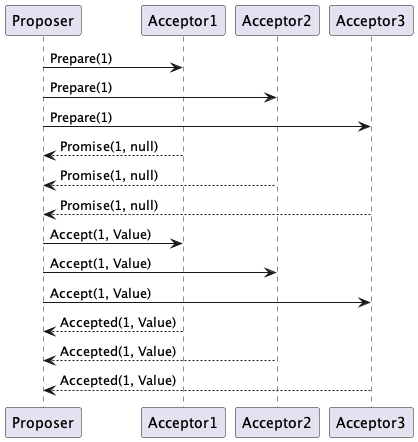
\includegraphics[width=0.55\textwidth]{fig/uml/paxos-default}
  \caption{Einfach Paxos als Beispielsequenze}
  \label{fig:simple-paxos}
\end{figure}


In diesem Diagramm sendet der Antragsteller (Proposer) zuerst eine Prepare-Anfrage an alle Akzeptoren. Die Akzeptoren antworten mit einem Versprechen (Promise). Dann sendet der Antragsteller eine Accept-Anfrage an alle Akzeptoren. Schließlich antworten die Akzeptoren mit einer Accepted-Nachricht, die signalisiert, dass sie den Vorschlag akzeptiert haben.

Paxos, obwohl es ein robustes und effizientes Protokoll ist, ist nicht ohne seine Herausforderungen. Es gibt mehrere kritische Szenarien, die bei der Anwendung des Paxos-Protokolls auftreten können.
\begin{itemize}
\item Netzwerklatenz und -ausfälle: Paxos kann durch Netzwerklatenz und -ausfälle erheblich gestört werden. Da Paxos auf der Kommunikation zwischen Prozessen basiert, können Verzögerungen und Ausfälle im Netzwerk dazu führen, dass Nachrichten verspätet oder gar nicht ankommen. Dies kann dazu führen, dass das Protokoll in einen unbestimmten Zustand gerät, in dem kein Konsens erreicht werden kann.
\item Konkurrierende Antragsteller: Ein weiteres kritisches Szenario tritt auf, wenn es mehrere konkurrierende Antragsteller gibt, die gleichzeitig versuchen, einen Konsens zu erreichen. Wenn jeder Antragsteller ständig neue Vorschläge mit höheren Nummern erzeugt, kann das System in einen Zustand geraten, der als \enquote{Livestream} bezeichnet wird, in dem kein Vorschlag jemals von einer Mehrheit der Akzeptoren akzeptiert wird.
\item Prozessausfälle: Da Paxos in verteilten Systemen eingesetzt wird, können Prozessausfälle ein ernsthaftes Problem darstellen. Wenn ein Antragsteller oder ein Akzeptor ausfällt, kann das den Fortschritt des Protokolls behindern. Paxos kann zwar Ausfälle tolerieren und sich erholen, aber der Ausfall kann dennoch zu Verzögerungen bei der Erreichung des Konsenses führen.
\end{itemize}

Um diese Szenarien in einer Sequenz zu illustrieren, können wir das vorherige Diagramm modifizieren, um die Auswirkungen von Netzwerk- und Prozessausfällen zu zeigen:


\begin{figure}[!ht]
  \centering
  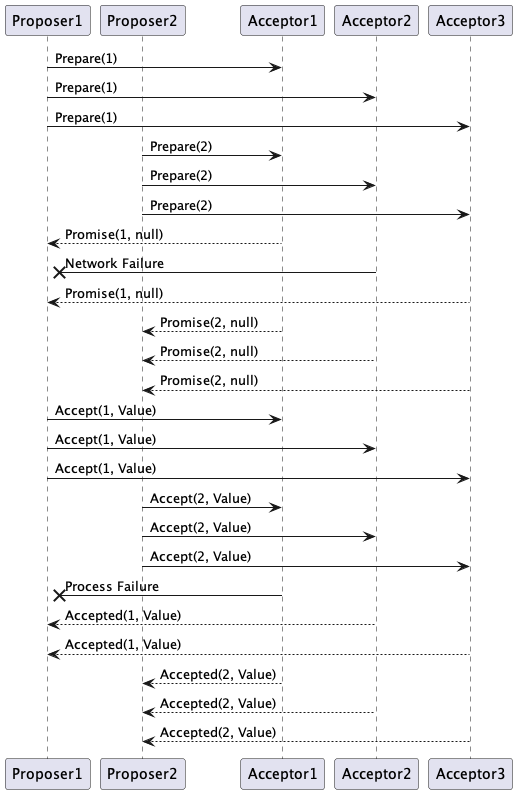
\includegraphics[width=0.65\textwidth]{fig/uml/paxos-issue}
  \caption{Komplexeres Paxos Beispiel}
  \label{fig:simple-paxos-issue}
\end{figure}

In diesem Diagramm sehen Sie, dass der Proposer1 eine Prepare-Anfrage an alle Akzeptoren sendet, aber die Anfrage an Acceptor2 scheitert aufgrund eines Netzwerkausfalls. Zur gleichen Zeit sendet Proposer2 auch Prepare-Anfragen, die alle erfolgreich sind. Proposer1 und Proposer2 senden dann ihre Accept-Anfragen, aber die Anfrage von Proposer1 an Acceptor1 scheitert wegen eines Prozessausfalls. Schließlich akzeptieren die Akzeptoren die Vorschläge von Proposer1 und Proposer2, aber aufgrund der Ausfälle gibt es keine Mehrheit, die einen einzigen Vorschlag akzeptiert, wodurch der Konsensprozess blockiert wird.

In der Realität würde in diesem kritischen Szenario Proposer1 den Konsens nicht erreichen, weil seine Accept-Anfrage an Acceptor1 aufgrund eines Prozessausfalls scheitert. Gleichzeitig würde Proposer2 erfolgreich Konsens erreichen, weil seine Accept-Anfragen von der Mehrheit der Akzeptoren akzeptiert werden.

Um die Situation zu beheben, könnte Proposer1 eine neue Runde mit einer höheren Vorschlagsnummer starten. Aber das würde zu weiterem Wettbewerb zwischen den Antragstellern führen und könnte das System in einen Zustand des \enquote{Livestreams} versetzen, in dem kein Konsens erreicht wird. Dieses Problem könnte durch den Einsatz eines Koordinators oder durch die Anwendung von Verzögerungen zur Begrenzung der Häufigkeit, mit der Antragsteller neue Runden starten, gemildert werden.

\begin{figure}[!htp]
  \centering
  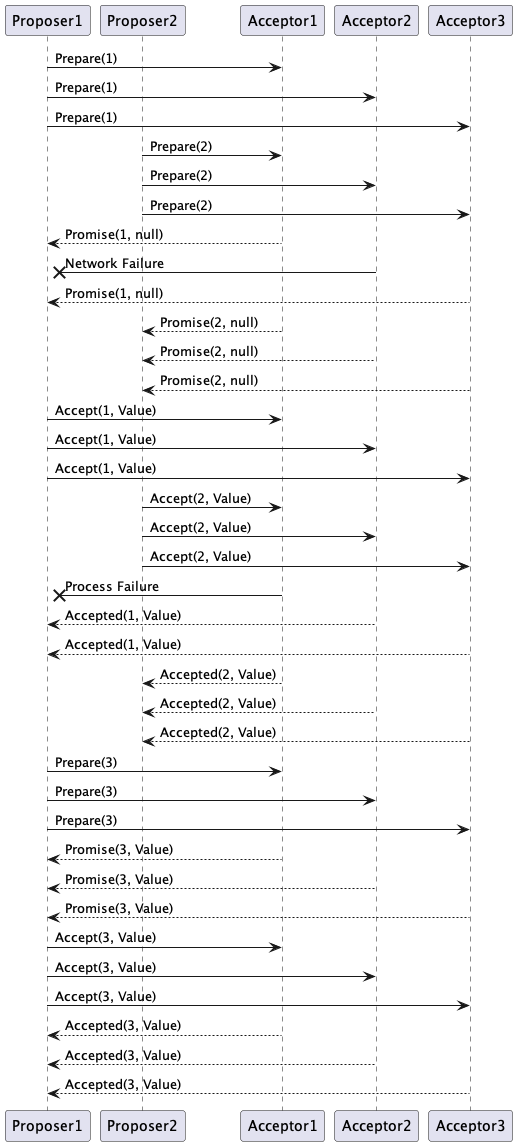
\includegraphics[width=0.65\textwidth]{fig/uml/paxos-issue-solve}
  \caption{Korrigiertes Paxos}
  \label{fig:simple-paxos-solve}
\end{figure}

In diesem Diagramm startet Proposer1 nach dem Ausfall eine neue Runde mit einer höheren Vorschlagsnummer und erreicht schließlich den Konsens.



\subsubsection{RAFT}\footnote{\url{https://www.youtube.com/watch?v=ro2fU8_mr2w}}

Das RAFT-Protokoll ist ein Konsensalgorithmus, der als Alternative zu Paxos entwickelt wurde. RAFT wurde entworfen, um die gleiche Funktionalität wie Paxos zu bieten, aber mit einem stärkeren Fokus auf Verständlichkeit und einfacher Implementierung.

Die wesentlichen Sequenzen in RAFT umfassen folgende Phasen:
\begin{itemize}
\item Wahl des Leaders: In RAFT gibt es immer einen Leader, der für die Koordination der Replikation verantwortlich ist. Wenn ein Knoten feststellt, dass es keinen Leader gibt (zum Beispiel, weil es keine Heartbeats vom Leader empfängt), beginnt es eine Wahl, indem es eine Anfrage zur Wahl an alle anderen Knoten sendet. Die Knoten stimmen für den ersten Kandidaten, der eine Anfrage sendet, und der Kandidat, der die meisten Stimmen erhält, wird zum neuen Leader.
\item Log-Replikation: Nachdem ein Leader gewählt wurde, beginnt der Prozess der Log-Replikation. Der Leader nimmt Anfragen von Clients entgegen, fügt sie seinem Log hinzu und sendet dann AppendEntries-Anfragen an die Follower, um das Log zu replizieren. Die Follower antworten dem Leader, wenn sie die Einträge erfolgreich repliziert haben.
\item Commit: Sobald der Leader feststellt, dass eine Mehrheit der Follower einen Log-Eintrag repliziert hat, erklärt er den Eintrag für committed und wendet den Eintrag auf seinen Zustand an. Der Leader informiert die Follower über committed Einträge durch nachfolgende AppendEntries-Anfragen.
\end{itemize}
Um diese Sequenzen in einer Sequenz zu illustrieren, wurde  das Diagramm XY angefertigt. In diesem Diagramm wird der Prozess der Leaderwahl, Log-Replikation und Commit in RAFT dargestellt.


\subsubsection{ZAB}
ZooKeeper Atomic Broadcast (ZAB) ist ein Konsensprotokoll, das von Apache ZooKeeper verwendet wird. Es ist darauf ausgelegt, eine geordnete, zuverlässige und atomare Übertragung von Nachrichten zwischen den Knoten eines verteilten Systems zu ermöglichen. Das ZAB-Protokoll hat zwei Hauptmodi: einen Erholungsmodus, der nach dem Ausfall eines Leaders ausgeführt wird, und einen Broadcast-Modus, der ausgeführt wird, wenn das System stabil ist.

Die wesentlichen Sequenzen von ZAB umfassen folgende Phasen:
\begin{itemize}
\item Führungsfindung (Leader Election): Wenn ein Leader ausfällt oder wenn das System zum ersten Mal startet, müssen die Knoten (die als \enquote{ZooKeeper Server} bezeichnet werden) einen neuen Leader wählen. Dies geschieht in der Phase der Führungsfindung, in der jeder Knoten einen Vorschlag mit seiner gewählten Führungsnummer (Epochennummer) und seiner eigenen Server-ID sendet. Der Knoten mit der höchsten gewählten Führungsnummer wird zum Leader.
\item Synchronisation: Nachdem ein Leader gewählt wurde, muss das System synchronisiert werden, um sicherzustellen, dass alle Knoten denselben Zustand haben. Der neue Leader sendet dazu seinen Zustand an alle anderen Knoten (Follower). Wenn ein Follower einen Zustand empfängt, der neuer als sein eigener ist, aktualisiert er seinen Zustand, um mit dem Leader übereinzustimmen.
\item Broadcast: Sobald das System synchronisiert ist, kann der Leader beginnen, Updates zu senden. Diese Updates werden als \enquote{Vorschläge} bezeichnet und enthalten eine eindeutige Transaktions-ID, die aus der Führungsnummer und einer fortlaufenden Sequenznummer besteht. Die Follower akzeptieren diese Vorschläge und fügen sie ihrem jeweiligen Zustand hinzu.
\end{itemize}

ZAB  ist somit  ein zuverlässiges, geordnetes und fehlertolerantes Protokoll, das dazu dient, Transaktionen auf mehrere Server zu verteilen, um eine fehlertolerante, verteilte Koordination zu ermöglichen. Es ist das zugrunde liegende Protokoll, das Apache ZooKeeper verwendet.

Im ZAB-Protokoll wird ein Leader-basiertes Multicast-Modell verwendet. In diesem Modell wird ein Knoten zum Leader gewählt, und dieser Leader ist verantwortlich für das Senden von Aktualisierungen an alle anderen Knoten (Follower) im Cluster. Der Leader garantiert die Reihenfolge der Nachrichten, was dazu beiträgt, eine \enquote{totale Ordnung} zu etablieren. Das bedeutet, dass alle Operationen, die im System auftreten, in einer konsistenten, vorhersehbaren Reihenfolge auftreten.

Dieses Modell ist zuverlässig, weil es sicherstellt, dass alle Nachrichten, die vom Leader gesendet werden, von den Followern empfangen werden. Wenn ein Follower eine Nachricht nicht empfängt, wird die Nachricht erneut gesendet, bis der Follower bestätigt, dass er sie empfangen hat.

Zusätzlich zur totalen Ordnung der vom Leader umgesetzten Nachrichten  unterstützt ZAB auch die kausale Ordnung der Operationen auf den Daten. Das bedeutet, dass wenn eine Operation A eine andere Operation B verursacht, Operation A immer vor Operation B in der Sequenz der Operationen auftreten wird.

In ZooKeeper sind die Garantien, die durch ZAB ermöglicht werden, sequenziell konsistent und atomar im Single Node Image. Das bedeutet, dass jede Operation, die auf einem Knoten ausgeführt wird, genau so aussieht, als ob sie auf einem einzelnen System ausgeführt wurde, und dass sie entweder vollständig ausgeführt wird oder überhaupt nicht.

ZooKeeper ermöglicht auch zeitnahe Operationen, wie das Erstellen, Löschen und Abrufen von Daten, sowie das Abrufen von Kindknoten. Diese Operationen werden in einem hierarchischen Namensraum ausgeführt, der es Entwicklern ermöglicht, Ressourcen auf eine strukturierte und organisierte Weise zu verwalten.

ZooKeeper bietet eine Vielzahl von Funktionen, die für verteilte Systeme tels unerlässlich sind, wie z.B.:
\begin{itemize}
\item Locks: ZooKeeper kann verwendet werden, um exklusive Sperren in einem verteilten System zu implementieren. Dies ist nützlich, wenn nur ein Prozess zu einem bestimmten Zeitpunkt eine Ressource verwenden darf.
\item Leader Election: In einigen verteilten Systemen kann es nötig sein, einen Prozess auszuwählen, der bestimmte Aufgaben ausführt. ZooKeeper kann verwendet werden, um diesen Leader auf einer fairen und transparenten Weise zu wählen.
\item Configuration Management: ZooKeeper kann verwendet werden, um Konfigurationsinformationen auf einer zentralen Stelle zu speichern und zu verteilen. Dies ist nützlich, um sicherzustellen, dass alle Prozesse in einem verteilten System die gleiche Konfiguration verwenden.
\end{itemize}

Das ZAB-Protokoll spielt dabei eine Schlüsselrolle, da es die konsistente und zuverlässige Ausführung dieser Funktionen ermöglicht. Durch die Verwendung von Leader-basiertem Multicast und der Gewährleistung von totaler und kausaler Ordnung stellt ZAB sicher, dass alle Prozesse in einem verteilten System eine konsistente Sicht auf die Daten haben.

Um zuverlässigen Datenverkehr zu gewährleisten, verwendet ZAB ein Zwei-Phasen-Commit-Protokoll, welches aus den Dantenbankgrundlagen bekannt sein sollte. Wenn ein Leader eine Aktualisierung vorschlägt, sendet er zunächst einen Vorschlag an alle Follower. Die Follower antworten dann mit einer Bestätigung, dass sie den Vorschlag erhalten haben. Erst wenn der Leader Bestätigungen von einer Mehrheit der Follower erhalten hat, kann er die Aktualisierung abschließen und an alle Follower senden.

All dies zusammen ermöglicht es ZooKeeper, eine konsistente und zuverlässige Koordination in verteilten Systemen zu gewährleisten. Es stellt sicher, dass alle Prozesse die gleiche Sicht auf die Daten haben und dass alle Operationen in einer konsistenten und vorhersehbaren Reihenfolge ausgeführt werden. 

\subsubsection{Konsens mit Crash Failures}
Die \enquote{Unmöglichkeit von 1-Crash-Konsens} in verteilten Systemen bezieht sich auf einen fundamentalen Beweis in der Theorie verteilter Systeme, der ursprünglich von Michael J. Fischer, Nancy A. Lynch und Michael S. Paterson in ihrem 1985 veröffentlichten Artikel \enquote{Impossibility of Distributed Consensus with One Faulty Process} vorgebracht wurde. Dieser Beweis wird oft als FLP-Unmöglichkeitstheorem bezeichnet.

Die grundlegende Aussage dieses Beweises ist, dass es in einem asynchronen verteilten System mit nur einem möglicherweise fehlerhaften Prozess (d.h. einem Prozess, der abstürzen kann) keinen deterministischen Algorithmus geben kann, der immer zu einem Konsens führt. Ein asynchrones System ist ein System, in dem es keine festen Obergrenzen für die Zeit gibt, die zum Senden von Nachrichten oder zum Ausführen von Schritten in einem Algorithmus benötigt wird.

Der Beweis nutzt die Tatsache, dass in einem asynchronen System immer die Möglichkeit besteht, dass ein Prozess oder eine Nachricht unendlich verzögert wird. Dies kann dazu führen, dass die anderen Prozesse nicht in der Lage sind, zu bestimmen, ob ein Prozess abgestürzt ist oder einfach nur verzögert wird. Daher kann es Fälle geben, in denen das System nicht in der Lage ist, einen Konsens zu erreichen, da es immer Unsicherheit darüber gibt, ob alle Prozesse ihren Zustand gemeldet haben oder nicht.

Dieses Ergebnis hat tiefgreifende Auswirkungen auf die Art und Weise, wie wir verteilte Systeme entwerfen und verstehen. Es zeigt, dass wir in bestimmten Fällen Kompromisse eingehen müssen, zum Beispiel indem wir die Asynchronität einschränken oder nichtdeterministische Algorithmen verwenden, um Konsens zu erreichen.

Die FLP-Unmöglichkeitsergebnisse haben zu einem tiefgreifenden Verständnis der Herausforderungen bei der Entwicklung von Algorithmen für verteilte Systeme geführt, insbesondere solchen, die Asynchronität und Fehler tolerieren müssen.

Die Schlussfolgerungen des FLP-Theorems haben die Forschung in mehrere Richtungen gelenkt:
\begin{itemize}
\item Teilsynchrone Systeme: In der Praxis sind Systeme selten völlig asynchron. Es gibt oft zumindest einige Grenzen für die Zeit, die Prozesse und Nachrichten benötigen. Dies hat zur Entwicklung von Konsensalgorithmen für teilsynchrone Systeme geführt, in denen bestimmte zeitliche Einschränkungen gelten, auch wenn sie recht locker sein können.
\item Randomisierte Algorithmen: Während das FLP-Ergebnis für deterministische Algorithmen gilt, ist es möglich, Konsens in einem asynchronen System zu erreichen, wenn wir Zufallszahlen einsetzen. Ein Beispiel für einen solchen Algorithmus ist der Randomized Consensus Algorithmus.
\item Praktische Konsensalgorithmen: Trotz des FLP-Unmöglichkeitsergebnisses wurden mehrere praktische Konsensalgorithmen für verteilte Systeme entwickelt, darunter Paxos, Raft und Zab. Diese Algorithmen sind entworfen, um in realen Systemen gut zu funktionieren, auch wenn sie in extrem asynchronen Szenarien oder bei bestimmten Arten von Netzwerkpartitionen scheitern können.
\end{itemize}
Es ist wichtig zu beachten, dass das FLP-Unmöglichkeitsergebnis spezifisch für asynchrone, unzuverlässige Systeme gilt. In einem synchronen System, in dem es feste Obergrenzen für die Zeit gibt, die Prozesse und Nachrichten benötigen, ist es möglich, einen Konsens zu erreichen, selbst wenn einige Prozesse abstürzen können. Gleiches gilt für asynchrone Systeme, in denen alle Prozesse zuverlässig sind. Das FLP-Ergebnis zeigt jedoch, dass die Kombination von Asynchronität und Unzuverlässigkeit zu grundlegenden Schwierigkeiten bei der Erzielung eines Konsenses führt.

Sowohl Bracha-Toueg als auch Chandra-Toueg sind Algorithmen, die versuchen, den Konsens in verteilten Systemen trotz der Einschränkungen, die durch das FLP-Unmöglichkeitsergebnis hervorgehoben wurden, zu erreichen. Beide Algorithmen nutzen das Konzept der teilweisen Synchronität, bei dem einige Obergrenzen für die Kommunikations- und Verarbeitungszeiten existieren, auch wenn diese Grenzen recht locker sind.
\begin{itemize}
\item Bracha-Toueg Crash Consensus: Dies ist ein Algorithmus für den binären Konsens in einem teilweise synchronen Modell, bei dem jeder Prozess entweder abstürzen kann (d.h., er kann zu irgendeinem Zeitpunkt aufhören, Aktionen auszuführen) oder korrekt ist. Der Bracha-Toueg-Algorithmus garantiert sowohl Sicherheit (d.h., alle korrekten Prozesse einigen sich auf den gleichen Wert, und wenn alle korrekten Prozesse den gleichen anfänglichen Wert haben, dann einigen sie sich auf diesen Wert) als auch Liveness (d.h., alle korrekten Prozesse entscheiden sich schließlich), solange mehr als zwei Drittel der Prozesse korrekt sind.
\item Chandra-Toueg Unreliable Failure Detectors: Dieser Ansatz konzentriert sich auf die Implementierung von Konsensalgorithmen in asynchronen Systemen mithilfe von sogenannten unzuverlässigen Fehlerdetektoren. Ein unzuverlässiger Fehlerdetektor ist ein Mechanismus, der die Möglichkeit hat, fehlerhafte Prozesse zu erkennen, aber Fehler machen kann, zum Beispiel indem er einen korrekten Prozess fälschlicherweise als fehlerhaft markiert. Chandra und Toueg zeigten, dass es möglich ist, mit solchen unzuverlässigen Fehlerdetektoren einen Konsens zu erzielen, auch in vollständig asynchronen Systemen.
\end{itemize}    

Unzuverlässige Fehlerdetektoren sind eine zentrale Komponente in vielen Algorithmen für verteilte Systeme, insbesondere in Konsensalgorithmen. Sie stellen eine Abstraktion dar, die es den Prozessen in einem verteilten System ermöglicht, zu erahnen, ob andere Prozesse abgestürzt sind.

Es ist wichtig zu beachten, dass Fehlerdetektoren als \enquote{unzuverlässig} bezeichnet werden, weil sie in asynchronen Systemen nicht perfekt sein können. In einem asynchronen System kann ein Prozess, der sehr langsam ist oder dessen Nachrichten stark verzögert werden, von anderen Prozessen als abgestürzt wahrgenommen werden, auch wenn er tatsächlich noch läuft.

Ein einfaches Beispiel für einen unzuverlässigen Fehlerdetektor ist ein Timeout-basierter Fehlerdetektor. In diesem Szenario würde jeder Prozess regelmäßig \enquote{Herzschlag}-Nachrichten an die anderen Prozesse senden. Wenn ein Prozess für eine bestimmte Zeit keine Herzschlag-Nachricht von einem anderen Prozess erhält, könnte er annehmen, dass dieser Prozess abgestürzt ist und ihn als solchen markieren.

Allerdings könnte ein sehr langsamer Prozess oder Netzwerkverzögerungen dazu führen, dass ein Prozess fälschlicherweise als abgestürzt markiert wird, wenn er tatsächlich noch funktioniert - daher die Bezeichnung \enquote{unzuverlässig}.

\subsubsection{Konsens mit Byzantine Failures}
In verteilten Systemen bezieht sich ein \enquote{byzantinischer Fehler} auf einen Fehler, der dazu führt, dass ein Knoten (oder Prozess) in einem System auf eine unvorhersehbare, unzuverlässige oder gar bösartige Weise reagiert. Der Begriff geht auf das berühmte \enquote{Byzantinische Generäle Problem} zurück, das ursprünglich in einem Artikel von Leslie Lamport, Robert Shostak und Marshall Pease aus dem Jahr 1982 formuliert wurde.

Das \enquote{Byzantinische Generäle Problem} ist ein Analogon zu den Herausforderungen, die bei der Koordination und dem Erreichen eines Konsenses in einem verteilten System auftreten, in dem einige der Knoten fehlerhaft sein könnten. Insbesondere müssen die \enquote{loyalen} Generäle (analog zu den korrekten Knoten in einem verteilten System) eine gemeinsame Strategie festlegen, trotz der Möglichkeit, dass einige der Generäle \enquote{Verräter} sein könnten und versuchen könnten, die loyale Koordination zu stören.

In einem verteilten System kann ein byzantinischer Knoten falsche oder inkonsistente Informationen an die anderen Knoten senden, kann scheinbar abstürzen und dann wieder auftauchen, oder kann auf andere Weise versuchen, die korrekte Funktion des Systems zu stören. Ein byzantinischer Fehler ist daher schwieriger zu handhaben als einfache Crash-Fehler, bei denen ein Knoten einfach aufhört zu reagieren.

Es wurde gezeigt, dass das Erreichen eines Konsenses in einem verteilten System mit byzantinischen Fehlern nur möglich ist, wenn mehr als zwei Drittel der Knoten korrekt sind. Es gibt verschiedene Algorithmen, die versuchen, dies zu erreichen, einschließlich der ursprünglichen Lösung, die in dem Artikel über die byzantinischen Generäle vorgeschlagen wurde, sowie späterer Algorithmen wie Practical Byzantine Fault Tolerance (PBFT).

Die Fähigkeit, byzantinische Fehler zu tolerieren, ist besonders wichtig in offenen, dezentralisierten Systemen wie Blockchains, in denen Knoten möglicherweise einen Anreiz haben, das System zu betrügen oder zu stören. Daher sind byzantinische Konsensalgorithmen ein aktiver Bereich der Forschung und Entwicklung in solchen Systemen. Neben PBFT werden die genannten Verfahren um Proof of Work oder auch Proof of Stake wieder relevant.  

\subsection{Koordination}

Die Koordination in verteilten Systemen ist eine wichtige Herausforderung, da einzelne Komponenten unabhängig voneinander agieren und Informationen austauschen müssen, um gemeinsame Ziele zu erreichen. Es gibt verschiedene Ansätze und Techniken, um die Koordination zu ermöglichen. Im Folgenden wird eine Einführung in die Koordination mittels Algorithmen geben:

\subsubsection{Waves}
Wave-Algorithmen sind eine Klasse von Algorithmen in der Graphentheorie und werden oft in verteilten Systemen eingesetzt. Sie zeichnen sich dadurch aus, dass sie Informationen über Graphen (oder Netzwerke) verteilen, ähnlich wie Wellen sich in einem physischen Medium ausbreiten. Diese Algorithmen werden typischerweise zur Lösung von Problemen wie dem Erkennen von Knoten, der Synchronisation von Prozessen, der Suche nach kürzesten Pfaden, der Auffindung von Toten Knoten und der Bestimmung von Grapheneigenschaften eingesetzt.

Die Grundidee bei Wave-Algorithmen ist, dass ein Knoten eine \enquote{Welle} (in Form einer Nachricht) an seine Nachbarn sendet und diese Welle sich dann durch den Graphen ausbreitet, bis alle Knoten erreicht sind. Während dieser Ausbreitung kann jeder Knoten, der die Welle erhält, eine bestimmte Aktion ausführen, wie zum Beispiel seinen Zustand aktualisieren oder Informationen an die Welle anhängen.

Ein einfacher Beispiel-Wave-Algorithmus könnte wie folgt aussehen:
\begin{itemize}
\item Ein Startknoten sendet eine Welle an alle seine Nachbarn.
\item Jeder Knoten, der die Welle erhält, führt eine bestimmte Aktion aus (zum Beispiel aktualisiert er einen Zähler oder speichert eine Information) und sendet die Welle an alle seine Nachbarn, die die Welle noch nicht erhalten haben.
\item Dieser Prozess wiederholt sich, bis alle Knoten im Graphen die Welle erhalten und verarbeitet haben.
\end{itemize}
Es gibt viele verschiedene Varianten von Wave-Algorithmen, abhängig von den spezifischen Anforderungen des Problems, das gelöst werden soll. Einige Wave-Algorithmen können zum Beispiel mehrere Wellen gleichzeitig senden, während andere spezielle Techniken verwenden können, um die Ausbreitung der Welle zu steuern und zu optimieren.

Wave-Algorithmen können in einer Vielzahl von Anwendungen eingesetzt werden, einschließlich Netzwerk-Routing, Synchronisation von verteilten Systemen, Erkennung von Knoten und Verteilung von Ressourcen in einem Netzwerk. In all diesen Fällen ermöglichen sie eine effiziente und dezentralisierte Lösung, die gut auf große und dynamische Systeme skaliert.

Traversal-, Tree- und Echo-Algorithmen sind spezielle Klassen von Wave-Algorithmen, die in verteilten Systemen eingesetzt werden, um bestimmte Aufgaben auszuführen. Hier ist eine kurze Beschreibung und ein Vergleich der drei:
\begin{itemize}
\item Traversal-Algorithmus (Graph-Durchlauf-Algorithmus): \\Traversal-Algorithmen werden verwendet, um alle Knoten in einem Graphen zu besuchen. Das bekannteste Beispiel für diese Art von Algorithmen sind Tiefensuche (Depth-First Search, DFS) und Breitensuche (Breadth-First Search, BFS). Beide Algorithmen beginnen bei einem bestimmten Knoten und besuchen alle anderen Knoten durch \enquote{Wandern} entlang der Kanten des Graphen. DFS macht dies, indem es so weit wie möglich entlang jeder Verzweigung geht, bevor es zurückkehrt, während BFS alle Nachbarn eines Knotens besucht, bevor es zu den Nachbarn der Nachbarn geht. Diese Algorithmen sind hilfreich bei Aufgaben wie dem Finden eines Pfades zwischen zwei Knoten, dem Testen, ob ein Graph zusammenhängend ist, oder dem Finden von Kreisen in einem Graphen.
\item Tree-Algorithmus (Baumalgorithmus): \\Tree-Algorithmen sind eine spezielle Klasse von Traversal-Algorithmen, die dazu dienen, einen Spannbaum (einen Baum, der alle Knoten des Graphen verbindet, aber keine Kreise enthält) aus einem Graphen zu erzeugen. Ein bekanntes Beispiel ist der Algorithmus von Prim oder Kruskal, der verwendet wird, um einen minimalen Spannbaum zu erzeugen. Diese Art von Algorithmen kann besonders nützlich sein in Netzwerken, um redundante Verbindungen zu entfernen und dennoch sicherzustellen, dass alle Knoten miteinander verbunden sind.
\item Echo-Algorithmus: \\Der Echo-Algorithmus ist ein spezieller Wave-Algorithmus, der dazu dient, Informationen über ein verteiltes System zu sammeln und an einen zentralen Knoten zurückzusenden. Ein Knoten sendet eine Anfrage an alle seine Nachbarn und wartet auf deren Antworten. Wenn ein Knoten eine Anfrage erhält, sendet er die Anfrage weiter an alle seine Nachbarn und wartet auf deren Antworten. Sobald ein Knoten alle Antworten von seinen Nachbarn erhalten hat, verarbeitet er die Antworten und sendet eine einzige Antwort an den Knoten, von dem er die ursprüngliche Anfrage erhalten hat. Dieser Algorithmus wird oft verwendet, um Informationen wie die Gesamtzahl der Knoten in einem Netzwerk, den kürzesten Pfad zu einem bestimmten Knoten oder die Verfügbarkeit von Ressourcen zu sammeln.
\end{itemize}
Alle Algorithmen bieten jeweils verschiedene Methoden zur Verarbeitung und Sammlung von Informationen in einem Netzwerk, abhängig von den spezifischen Anforderungen der Aufgabe.

\subsubsection{Snapshot}

Snapshot-Algorithmen sind eine Art von Algorithmen in verteilten Systemen, die dazu verwendet werden, den globalen Zustand des Systems zu einem bestimmten Zeitpunkt zu erfassen. Diese Algorithmen sind besonders nützlich in Systemen, in denen verschiedene Prozesse gleichzeitig und unabhängig voneinander ausgeführt werden, da sie es ermöglichen, einen konsistenten \enquote{Schnappschuss} des Zustands aller Prozesse zu erstellen.

Es gibt verschiedene Snapshot-Algorithmen, aber einer der bekanntesten ist der Chandy-Lamport-Algorithmus. Dieser Algorithmus wurde 1985 von K. Mani Chandy und Leslie Lamport entwickelt. Der Algorithmus ermöglicht es, einen globalen Zustand eines verteilten Systems zu erfassen, der konsistent ist hinsichtlich \enquote{happen-before} Beziehungen zwischen Ereignissen.

Hier ist eine vereinfachte Beschreibung des Chandy-Lamport-Algorithmus:
\begin{itemize}
\item Ein Prozess, der einen globalen Zustandsschnappschuss initiieren möchte (wir nennen ihn Initiator), speichert seinen eigenen Zustand und sendet spezielle Marker-Nachrichten an alle anderen Prozesse, mit denen er kommuniziert.
\item Wenn ein Prozess eine Marker-Nachricht erhält und es ist das erste Mal, dass er einen Marker für diesen Schnappschuss erhält, speichert er seinen aktuellen Zustand und sendet Marker-Nachrichten an alle anderen Prozesse, mit denen er kommuniziert. Außerdem beginnt er, alle eingehenden Nachrichten auf jedem Kanal zu speichern, bis er einen Marker auf diesem Kanal erhält.
\item Wenn ein Prozess eine Marker-Nachricht auf einem Kanal erhält und er hat bereits seinen Zustand für diesen Schnappschuss gespeichert, stoppt er die Aufzeichnung der Nachrichten auf diesem Kanal.
\end{itemize} 
Nachdem der Algorithmus ausgeführt wurde, besteht der Schnappschuss aus dem gespeicherten Zustand jedes Prozesses und den gespeicherten Nachrichten auf jedem Kanal. Dieser Schnappschuss ist konsistent im Sinne von \enquote{happen-before} Beziehungen: Wenn ein Ereignis A vor einem Ereignis B auftritt, dann wird, wenn der Schnappschuss nach B aufgenommen wird, auch A im Schnappschuss enthalten sein.


Neben dem Chandy-Lamport-Algorithmus existieren andere Algorithmen, wie der Lai-Yang-Algorithmus. Dieser unterscheidet sich jedoch in der Art und Weise, wie er das Ziel erreicht.

Der Chandy-Lamport-Algorithmus setzt auf die Verwendung von Marker-Nachrichten, die zwischen den Prozessen hin und her geschickt werden, um den Start- und Endpunkt der Schnappschusserfassung zu signalisieren. Wenn ein Prozess eine Marker-Nachricht erhält, speichert er seinen Zustand und leitet die Marker-Nachricht an alle seine Ausgangskanäle weiter. Dieser Prozess wird fortgesetzt, bis alle Prozesse ihren Zustand gespeichert und alle Marker-Nachrichten erhalten haben. Ein wichtiger Aspekt dieses Algorithmus ist, dass er einen synchronisierten Startpunkt erfordert, aber keinen synchronisierten Endpunkt.

Der Lai-Yang-Algorithmus hingegen ist ein sogenannter \enquote{farbiger} Algorithmus. In diesem Kontext bedeutet \enquote{farbig}, dass Nachrichten und Prozesse entweder als \enquote{rot} oder \enquote{weiß} markiert sind. Zu Beginn des Algorithmus sind alle Prozesse und Nachrichten weiß. Wenn ein Prozess beschließt, einen Schnappschuss zu starten, wird er rot und speichert seinen Zustand. Es sendet dann rote Nachrichten an alle anderen Prozesse. Ein Prozess, der eine rote Nachricht erhält, speichert seinen Zustand und wird ebenfalls rot. 
Im Detail ist der Algorithmus wie folgt:
\begin{itemize}
\item Initialisierung: Zu Beginn des Algorithmus sind alle Prozesse und Nachrichten weiß.
\item Start des Snapshots: Ein beliebiger Prozess kann die Aufnahme eines Schnappschusses initiieren. Dieser Prozess ändert seine Farbe von Weiß zu Rot, speichert seinen lokalen Zustand und beginnt, rote Nachrichten zu senden.
\item Aufnahme des Zustands: Wenn ein weißer Prozess eine rote Nachricht empfängt, ändert er seine Farbe zu Rot, speichert seinen lokalen Zustand und beginnt, rote Nachrichten zu senden. Wenn ein roter Prozess eine rote Nachricht empfängt, ändert er nichts an seinem Zustand, sondern sendet weiterhin rote Nachrichten.
\item Ende des Snapshots: Der globale Zustand des Systems ist erfasst, sobald alle Prozesse rot geworden sind und alle weißen Nachrichten aus dem System entfernt wurden. Da alle roten Prozesse nur rote Nachrichten senden, werden alle Nachrichten, die nach dem Snapshot empfangen werden, ebenfalls rot sein.
\end{itemize}

Es ist wichtig zu beachten, dass dieser Algorithmus auch sicherstellt, dass der erfasste globale Zustand des Systems konsistent ist, d.h., er respektiert die \enquote{happen-before}-Beziehungen zwischen den Ereignissen im System.  Der Vorteil dieses Algorithmus besteht darin, dass er keinen synchronisierten Startpunkt erfordert, was ihn flexibler macht als den Chandy-Lamport-Algorithmus. Allerdings kann er mehr Ressourcen verbrauchen, insbesondere in Systemen mit vielen Prozessen und Nachrichten.

Anwendungen von Snapshot-Algorithmen sind:
\begin{itemize}
\item Deadlock-Erkennung: Snapshot-Algorithmen können verwendet werden, um Deadlocks in verteilten Systemen zu erkennen. Durch die Erfassung des globalen Zustands des Systems kann ein Prozess bestimmen, ob es eine Zyklusabhängigkeit zwischen Prozessen gibt, was auf einen Deadlock hindeuten würde.
\item Globales Checkpointing: In verteilten Systemen kann ein globaler Schnappschuss dazu verwendet werden, einen Zustand zu erzeugen, zu dem das System nach einem Ausfall zurückkehren kann. Dies ist nützlich, um die Ausfallerholung zu erleichtern und den Datenverlust zu minimieren.
\item Eventuelle Konsistenz: Snapshot-Algorithmen können verwendet werden, um sicherzustellen, dass eine verteilte Datenbank im Laufe der Zeit eine konsistente Ansicht der Daten erreicht. Mit anderen Worten, sie können dazu beitragen, sicherzustellen, dass alle Repliken eines Datenelements schließlich denselben Wert haben.
\item Monitoring und Debugging: In verteilten Systemen kann es eine Herausforderung sein, die Interaktionen zwischen den verschiedenen Prozessen zu verstehen, insbesondere wenn Probleme auftreten. Durch die Aufnahme eines globalen Schnappschusses des Systems zu einem bestimmten Zeitpunkt können Entwickler oder Systemadministratoren den Zustand jedes Prozesses und die Nachrichten, die zwischen den Prozessen ausgetauscht werden, überprüfen. Dies kann dabei helfen, das Problem zu identifizieren und zu beheben.
\item Simulation von verteilten Systemen: Snapshot-Algorithmen können auch in der Simulation von verteilten Systemen nützlich sein. Durch die Aufnahme von Schnappschüssen des Systems zu verschiedenen Zeitpunkten können Wissenschaftler das Verhalten des Systems unter verschiedenen Bedingungen analysieren und besser verstehen.
\item Konsistenz in verteilten Datenbanken: Snapshot-Algorithmen können dazu beitragen, konsistente Lesevorgänge in verteilten Datenbanken zu ermöglichen, indem sie eine konsistente Ansicht der Datenbank zu einem bestimmten Zeitpunkt erzeugen. Dies ist besonders wichtig in Systemen, die eine hohe Verfügbarkeit und Partitionstoleranz erfordern.
\end{itemize}

\subsubsection{Checkpoint}
Der Peterson-Kearns Rollback Recovery-Algorithmus unterscheidet sich von den beiden anderen Algorithmen, da er nicht nur darauf abzielt, den globalen Zustand eines Systems zu erfassen, sondern auch darauf, das System zu einem konsistenten Zustand zurückzusetzen, wenn ein Fehler auftritt. Er tut dies, indem er sogenannte \enquote{Checkpoints} oder gespeicherte Zustände der Prozesse verwendet. Wenn ein Fehler erkannt wird, wird das System zu dem Checkpoint zurückgesetzt, der unmittelbar vor dem Fehler auftrat. Dann wird das System von diesem Punkt aus neu gestartet, wobei alle Nachrichten, die nach dem Checkpoint empfangen wurden, erneut gesendet werden. Dieser Ansatz kann effektiv sein, um die Ausfallzeit in einem verteilten System zu minimieren, erfordert aber ein sorgfältiges Management der Checkpoints und der Nachrichtenwiederholung.
Im Detail ist der Algorithmus wie folgt:
\begin{itemize}
\item Checkpointing: Jeder Prozess im System führt in regelmäßigen Abständen ein lokales Checkpointing durch, bei dem der aktuelle Zustand des Prozesses gespeichert wird. Diese Checkpoints dienen als Wiederherstellungspunkte im Falle eines Fehlers.
\item Nachrichtenprotokollierung: Zusätzlich zum Checkpointing protokolliert jeder Prozess alle gesendeten und empfangenen Nachrichten. Dies ermöglicht es dem System, den genauen Zustand zum Zeitpunkt des letzten Checkpoints zu rekonstruieren.
\item Fehlererkennung: Wenn ein Fehler in einem Prozess erkannt wird, wird dieser Prozess und möglicherweise auch andere Prozesse, die von dem fehlerhaften Prozess abhängig sind, zu ihrem letzten Checkpoint zurückgerollt.
\item Nachrichtenwiederholung: Nach dem Rollback werden alle Nachrichten, die nach dem letzten Checkpoint gesendet wurden, aus dem Protokoll erneut gesendet. Dies stellt sicher, dass alle Prozesse, die von dem fehlerhaften Prozess abhängig sind, wieder in einen konsistenten Zustand gebracht werden.
\item Wiederherstellung: Nachdem alle Nachrichten wiederholt wurden, wird der Betrieb des Systems fortgesetzt.
\end{itemize}
Der Peterson-Kearns-Rollback-Recovery-Algorithmus hat den Vorteil, dass er es ermöglicht, das System nach einem Fehler schnell zu einem konsistenten Zustand zurückzusetzen. Dies kann dazu beitragen, die Ausfallzeit des Systems zu minimieren und den Datenverlust zu begrenzen. Allerdings erfordert dieser Ansatz ein sorgfältiges Management der Checkpoints und der Nachrichtenprotokollierung, und er kann zu einer erheblichen Wiederholung von Berechnungen führen, wenn Fehler auftreten.


\subsubsection{Deadlock Detection}

Deadlocks sind Situationen in verteilten Systemen (und auch in anderen Arten von Systemen), in denen zwei oder mehr Prozesse unbegrenzt auf Ressourcen warten, die von den anderen Prozessen gehalten werden. Deadlock-Erkennungsalgorithmen sind Verfahren, die entwickelt wurden, um diese Situationen zu identifizieren und gegebenenfalls zu beheben.

Ein grundlegender Ansatz zur Deadlock-Erkennung besteht darin, den Ressourcenzuteilungsgraphen des Systems zu überprüfen. Dieser Graph besteht aus Knoten, die Prozesse und Ressourcen darstellen, und Kanten, die die Beziehungen zwischen diesen Elementen (z.B. \enquote{Prozess P besitzt Ressource R} oder \enquote{Prozess P wartet auf Ressource R}) 
darstellen. Ein Deadlock tritt auf, wenn es in diesem Graphen einen Zyklus gibt. Das bedeutet, dass es eine Gruppe von Prozessen gibt, in der jeder Prozess auf eine Ressource wartet, die von einem anderen Prozess in der Gruppe gehalten wird.
Zur Erkennung von Deadlocks in verteilten Systemen gibt es verschiedene Algorithmentypen. Hier sind zwei gängige Methoden:

\begin{itemize}
\item Wait-for-Graphs-Algorithmus: Wait-for-Graphs sind eine gängige Methode zur Deadlock-Erkennung in Betriebssystemen und verteilten Systemen. Sie stellen die Abhängigkeiten zwischen Prozessen und Ressourcen dar. Knoten im Graphen repräsentieren Prozesse und Ressourcen, während Kanten die \enquote{wartet auf} Beziehungen darstellen. Wenn ein Prozess auf eine Ressource wartet, die von einem anderen Prozess gehalten wird, wird eine Kante von dem wartenden Prozess zum haltenden Prozess gezeichnet. Ein Zyklus in diesem Graphen deutet auf einen Deadlock hin, da jeder Prozess im Zyklus auf eine Ressource wartet, die von einem anderen Prozess im Zyklus gehalten wird. Dieser Algorithmus wird typischerweise in einem zentralisierten System verwendet, in dem ein einziger Koordinator den gesamten Wait-for-Graphen aufbewahrt und auf Deadlocks prüft. In einem verteilten System könnte ein ähnlicher Ansatz mit einem verteilten Graphen und einer koordinierten Zykluserkennung verwendet werden.
\item Konsensbasierte Algorithmen sind eine Art von Koordinationsmechanismus, der oft in verteilten Systemen verwendet wird. Sie ermöglichen es den Knoten (Prozessen) in einem verteilten System, sich auf einen gemeinsamen Wert oder Zustand zu einigen, auch wenn einige Knoten fehlerhaft sein können oder es Netzwerkverzögerungen gibt.

In Bezug auf Deadlock-Erkennung in verteilten Systemen könnten konsensbasierte Algorithmen auf verschiedene Weisen genutzt werden:
\begin{itemize}
\item Gemeinsame Sicht auf Systemzustand: Jeder Knoten könnte seine lokale Sicht auf den Zustand des Systems (z.B. seine \enquote{wartet auf} Beziehungen oder gehaltenen Ressourcen) mit den anderen Knoten teilen. Die Knoten könnten dann einen Konsensalgorithmus verwenden, um eine gemeinsame Sicht auf den gesamten Systemzustand zu erzielen.
\item Entscheidung über Deadlock-Zustand: Nachdem ein gemeinsamer Systemzustand erzielt wurde, könnten die Knoten einen weiteren Konsensalgorithmus verwenden, um sich darauf zu einigen, ob ein Deadlock vorliegt oder nicht. Dies könnte zum Beispiel durch Suche nach Zyklen in einem gemeinsamen Wait-for-Graphen geschehen.
\item Handhabung von Deadlocks: Wenn ein Deadlock erkannt wird, könnten die Knoten einen Konsensalgorithmus verwenden, um zu entscheiden, wie der Deadlock aufgelöst werden sollte (z.B. welcher Prozess zurückgesetzt werden sollte oder welche Ressourcen freigegeben werden sollten).
\end{itemize}    
\end{itemize}

Es ist wichtig zu beachten, dass diese Algorithmen unterschiedliche Anforderungen an die Systeme haben, in denen sie eingesetzt werden. Der Wait-for-Graphs-Algorithmus setzt voraus, dass genaue und aktuelle Informationen über alle Prozesse und Ressourcen im System verfügbar sind, während der konsensbasierter Algorithmus darauf ausgelegt ist, in Systemen zu arbeiten, in denen diese Informationen möglicherweise unvollständig oder verzögert sind. Darüber hinaus ist der konsensbasierter Algorithmus fehlertolerant, während der Wait-for-Graphs-Algorithmus in der Regel nicht mit Prozessausfällen umgehen kann.	

Diese Ansätze finden Anwendung in Verfahren wie:

\begin{itemize}
\item Chandy-Misra-Haas-Algorithmus: Dieser Algorithmus erfordert, dass jeder Prozess eine \enquote{Wartet auf}-Beziehung zu einem anderen Prozess einrichtet, wenn er eine Ressource anfordert, die von diesem Prozess gehalten wird. Wenn ein Prozess feststellt, dass er in einer Warteschleife ist, initiiert er eine Abfrage, die durch das Netzwerk wandert und Informationen über \enquote{Wartet auf}-Beziehungen sammelt. Wenn die Abfrage zum Initiator zurückkehrt, wird ein Deadlock festgestellt.
\item Menekes-Shoshani-Algorithmus: Dieser Algorithmus verwendet einen globalen Wait-for-Graphen, der periodisch auf Zyklusbedingungen überprüft wird. Wenn ein Zyklus gefunden wird, wird ein Deadlock festgestellt.
\item Bracha-Toueg-Algorithmus: Der Bracha-Toueg-Algorithmus ist ein konsensbasierter Algorithmus für verteilte Systeme, der unter anderem für die Deadlock-Erkennung verwendet werden kann. Er ist darauf ausgelegt, in einem asynchronen Netzwerk zu arbeiten, in dem Nachrichten unbestimmte Verzögerungen haben können und Prozesse unerwartet ausfallen können. Der Algorithmus ermöglicht es den Prozessen, einen Konsens über einen bestimmten Wert zu erreichen, indem sie Nachrichten austauschen und auf die Mehrheit der Antworten warten. Im Kontext der Deadlock-Erkennung könnte der Bracha-Toueg-Algorithmus verwendet werden, um einen Konsens über das Vorhandensein eines Deadlocks zu erreichen. Jeder Prozess könnte seine lokale Sicht auf den Zustand des Systems (z.B. seine \enquote{wartet auf} Beziehungen) mit den anderen teilen und dann auf der Grundlage der erhaltenen Informationen eine Entscheidung treffen.
\end{itemize}
Einmal erkannt, kann ein Deadlock oft durch Maßnahmen wie das Zurücksetzen oder Beenden eines oder mehrerer Prozesse, die Freigabe von Ressourcen oder das Umorganisieren der Ressourcenzuteilungen gelöst werden. Es ist jedoch zu beachten, dass diese Maßnahmen sorgfältig durchgeführt werden müssen, um unerwünschte Nebenwirkungen zu vermeiden.

Es ist auch wichtig zu bedenken, dass Deadlock-Erkennung in verteilten Systemen eine Herausforderung darstellen kann, da Informationen über den Zustand des gesamten Systems gesammelt und analysiert werden müssen. Darüber hinaus können Deadlocks in verteilten Systemen oft vermieden werden, indem geeignete Ressourcenzuteilungsstrategien und Kommunikationsprotokolle verwendet werden.



\subsubsection{Termination}
Terminierungserkennung ist ein wichtiger Aspekt in verteilten Systemen, bei dem es darum geht festzustellen, wann alle Prozesse in einem verteilten System ihre Ausführung abgeschlossen haben. Dies ist besonders nützlich bei Algorithmen, bei denen die Prozesse unabhängig voneinander arbeiten und sich gegenseitig keine direkten Signale senden, wenn sie ihre Aufgabe beendet haben.

Es gibt mehrere Algorithmen, die zur Erkennung der Terminierung in verteilten Systemen eingesetzt werden können. Im Folgenden werden zwei gängige Methoden beschrieben:
\begin{itemize}
\item Scholten's Algorithmus: Dieser Algorithmus basiert auf dem Konzept der \enquote{Wurzel} und der \enquote{Wellen}. Ein Initiator (Wurzel) startet den Algorithmus, indem er an alle Prozesse eine Anfrage sendet. Wenn ein Prozess eine Anfrage erhält, sendet er die Anfrage weiter an alle seine Nachbarn und wird zum \enquote{aktiven} Zustand. Wenn ein aktiver Prozess keine ausstehenden Anfragen mehr hat, sendet er eine Terminierungsnachricht (auch als \enquote{Echo} bekannt) an den Prozess, von dem er die ursprüngliche Anfrage erhalten hat. Der Initiator sammelt die Echos und wenn er alle erhalten hat, wird festgestellt, dass das System terminiert hat.
\item Dijkstra-Scholten-Algorithmus: Dies ist eine Verbesserung des Scholten's Algorithmus und verwendet ein Konzept namens \enquote{diffusing computation}. In diesem Ansatz sendet ein Prozess Anfragen nur an seine \enquote{Kinder} und nicht an alle anderen Prozesse. Wenn ein Kind fertig ist, sendet es eine Terminierungsnachricht an seinen \enquote{Eltern}-Prozess. Wenn ein Elternprozess von allen seinen Kindern Terminierungsnachrichten erhalten hat, sendet er selbst eine Terminierungsnachricht an seinen eigenen Elternprozess. Dies setzt sich fort, bis die Nachricht den Initiator erreicht, der dann feststellt, dass das System terminiert hat.
\item Rana's Algorithmus: Rana's Algorithmus ist ein einfacher und effizienter Ansatz zur Terminierungserkennung. Es basiert auf dem Versenden von \enquote{Probe}-Nachrichten von einem Prozess (dem Initiator) zu allen anderen Prozessen im System. Wenn ein Prozess eine Probe-Nachricht erhält und keine aktiven Aufgaben hat, sendet er eine Antwort zurück zum Initiator. Wenn der Initiator von allen Prozessen Antworten erhalten hat, wird die Terminierung des Systems festgestellt. Der Hauptvorteil dieses Algorithmus ist seine Einfachheit. Der Nachteil ist, dass er in großen Systemen ineffizient sein kann, da er erfordert, dass der Initiator mit jedem Prozess einzeln kommuniziert.
\item Safra's Algorithmus: Safra's Algorithmus ist ein ausgefeilterer Ansatz zur Terminierungserkennung, der auf der Verwendung von \enquote{Token}-Nachrichten basiert, die im System zirkulieren. Wenn ein Prozess eine Aufgabe abgeschlossen hat, sendet er das Token an den nächsten Prozess weiter. Wenn das Token den Initiator erreicht und alle Prozesse ihre Aufgaben abgeschlossen haben, wird die Terminierung des Systems festgestellt. Safra's Algorithmus ist effizient und benötigt eine geringe Anzahl von Nachrichten, um die Terminierung festzustellen. Allerdings ist er komplexer zu implementieren als Rana's Algorithmus.
\item Weight Throwing Algorithmus: Der Weight Throwing Algorithmus ist ein weiterer Ansatz zur Terminierungserkennung. Bei diesem Ansatz hat jeder Prozess ein \enquote{Gewicht}, das repräsentiert, wie viel Arbeit er noch zu erledigen hat. Wenn ein Prozess eine Aufgabe abschließt, \enquote{wirft} er einen Teil seines Gewichts an einen anderen Prozess. Wenn der Initiator ein Gewicht von null hat und keine Gewichte mehr empfängt, wird die Terminierung des Systems festgestellt. Der Weight Throwing Algorithmus kann effizient sein, insbesondere in Systemen, in denen die Arbeitslasten ungleich verteilt sind. Allerdings kann er in großen Systemen zu viel Kommunikation erfordern.
\item Fault Tolerant Weight Throwing: Dies ist eine Variante des Weight Throwing Algorithmus, die darauf ausgelegt ist, Fehler in verteilten Systemen zu tolerieren. Bei diesem Ansatz wird das \enquote{Gewicht} eines Prozesses auf mehrere andere Prozesse verteilt, um sicherzustellen, dass das Gewicht nicht verloren geht, wenn ein Prozess ausfällt. Dieser Algorithmus bietet eine höhere Fehlertoleranz als der ursprüngliche Weight Throwing Algorithmus, kann aber auch mehr Kommunikation erfordern.
\end{itemize}
Insgesamt hängt die Auswahl des besten Terminierungserkennungsalgorithmus von den spezifischen Anforderungen des Systems ab, einschließlich seiner Größe, der Verteilung der Arbeitslasten, der Anforderungen an die Fehlertoleranz und der verfügbaren Ressourcen für die Kommunikation.

\subsubsection{Garbage}
Garbage Collection (GC) in verteilten Systemen stellt eine größere Herausforderung dar als in einem einzelnen Rechner, da Objekte über verschiedene Knoten hinweg verteilt sein können und Kommunikation zwischen den Knoten erfordert wird, um zu bestimmen, ob ein Objekt gelöscht werden kann oder nicht. Im Folgenden werden einige bekannte Algorithmen für die Garbage Collection in verteilten Systemen vorgestellt:
\begin{itemize}
\item Referenzzählung: Dieser Ansatz ist einer der einfachsten für die Garbage Collection. Jedes Objekt hält eine Zählung aller Referenzen, die auf es zeigen. Wenn ein Objekt erstellt wird, wird seine Referenzzählung auf eins gesetzt. Wenn eine Referenz hinzugefügt wird, wird die Zählung inkrementiert und wenn eine Referenz entfernt wird, wird sie dekrementiert. Wenn die Zählung auf null fällt, ist das Objekt für die Garbage Collection bereit. Der Hauptnachteil dieses Ansatzes ist, dass er keine zyklischen Referenzen handhaben kann, d.h. wenn zwei oder mehr Objekte sich gegenseitig referenzieren, aber von keinem anderen Objekt im System referenziert werden.
\item Verteilte Mark-and-Sweep: Dieser Algorithmus ist eine Erweiterung des traditionellen Mark-and-Sweep Algorithmus für verteilte Systeme. In der Markierungsphase werden alle erreichbaren Objekte markiert, indem ausgehend von den Wurzelobjekten (d.h., Objekte, die direkt zugänglich sind, z.B. durch lokale Variablen in aktiven Funktionen) alle referenzierten Objekte traversiert werden. In der Sweep-Phase werden alle unmarkierten Objekte, die also nicht erreichbar sind, als Müll gesammelt. In einem verteilten System erfordert dies eine Kommunikation zwischen den Knoten, um zu bestimmen, welche Objekte erreichbar sind.
\item Zyklische Garbage Collection: Dieser Algorithmus ist eine Erweiterung der Referenzzählung, um zyklische Referenzen zu erkennen und zu sammeln. Dies kann erreicht werden, indem periodisch eine zyklische Referenzzählung durchgeführt wird, die bestimmt, ob es Objekte gibt, die nur durch einen Zyklus von Referenzen erreichbar sind. Diese Algorithmen können komplex sein und erfordern eine beträchtliche Kommunikation zwischen den Knoten, um zyklische Referenzen zu erkennen.
\item Garbage Collection mit Leases: Bei diesem Ansatz wird ein Timeout (oder \enquote{Lease}) für jede Referenz festgelegt. Wenn die Lease abläuft, wird die Referenz automatisch entfernt, es sei denn, sie wird erneuert. Dieser Ansatz kann in Systemen nützlich sein, in denen die Kommunikation zwischen den Knoten unzuverlässig ist oder in denen es akzeptabel ist, dass Objekte nach einer bestimmten Zeit automatisch gelöscht werden.
\item Verteilte Garbage Collection durch Tracing: Dieser Ansatz ähnelt dem Mark-and-Sweep-Algorithmus, nutzt aber Tracing, um die Erreichbarkeit von Objekten in einem verteilten System zu bestimmen. Dieser Ansatz kann effizienter sein, erfordert aber mehr Kommunikation zwischen den Knoten und kann daher in Netzwerken mit hoher Latenz weniger wirksam sein.
\item Generational Garbage Collection: In vielen Anwendungen ist die Lebensdauer von Objekten nicht gleichmäßig verteilt - viele Objekte werden kurz nach ihrer Erstellung nicht mehr benötigt, während andere über einen längeren Zeitraum bestehen bleiben. Generational Garbage Collection nutzt diese Tatsache aus, indem sie den Speicher in verschiedene \enquote{Generationen} aufteilt, basierend auf der Lebensdauer der Objekte. Junge Objekte werden häufiger auf Müll überprüft, während ältere Objekte seltener überprüft werden. Dies kann die Effizienz der Garbage Collection erheblich verbessern, erfordert aber eine sorgfältige Verwaltung der Generationen und kann bei falscher Anwendung zu Speicherlecks führen.
\end{itemize}
Insgesamt ist die Auswahl des besten Garbage Collection Algorithmus für ein verteiltes System eine komplexe Aufgabe, die eine gründliche Kenntnis der Systemarchitektur und der Anwendungsanforderungen erfordert. Es ist auch wichtig, die Leistung des ausgewählten Algorithmus regelmäßig zu überwachen und anzupassen, um sicherzustellen, dass er effektiv und effizient bleibt.

\subsubsection{Election}
Es gibt viele Algorithmen zur Durchführung von Wahlen in verteilten Systemen. Die Wahl ist ein grundlegender Prozess in verteilten Systemen, der dazu dient, einen Koordinator oder Leader zu wählen. Hier sind einige der wichtigsten Wahlalgorithmen und ihre Arbeitsweise:
\begin{itemize}
\item Election in Rings (Ring Election Algorithmus): Dieser Algorithmus wird in Systemen mit einer Ringstruktur verwendet. Ein Knoten, der feststellt, dass der Koordinator ausgefallen ist, beginnt eine Wahl, indem er eine Wahlmeldung an den nächsten Knoten im Ring sendet. Diese Nachricht enthält die ID des wählenden Knotens. Jeder Knoten, der die Wahlmeldung erhält, fügt seine ID hinzu und leitet die Nachricht weiter. Wenn die Wahlmeldung zu ihrem Ursprungsknoten zurückkehrt, wird der Knoten mit der höchsten ID als Koordinator ausgewählt.
\item Bully Algorithmus: In diesem Algorithmus beginnt jeder Knoten, der erkennt, dass der Koordinator ausgefallen ist, eine Wahl. Der Knoten sendet eine Wahlmeldung an alle anderen Knoten mit höheren IDs. Wenn er keine Antwort erhält, erklärt er sich selbst zum Koordinator. Wenn er jedoch eine Antwort von einem Knoten mit einer höheren ID erhält, wird er zum \enquote{Unterdrückten} und wartet auf eine Nachricht von dem Knoten, der sich zum Koordinator erklärt.
\item Tree Election Algorithmus: Dieser Algorithmus verwendet eine Baumstruktur, um die Wahl durchzuführen. Der Baum ist so organisiert, dass der Knoten mit der höchsten ID an der Wurzel steht. Wenn ein Knoten feststellt, dass der Koordinator ausgefallen ist, sendet er eine Wahlmeldung an den Wurzelknoten. Der Wurzelknoten wählt dann den Knoten mit der höchsten ID als neuen Koordinator.
\item Echo-Algorithmus mit Ausnahmen: Der Echo-Algorithmus ist ein grundlegender Algorithmus für verteilte Systeme, der verwendet werden kann, um Informationen in einem Netzwerk zu verbreiten oder eine globale Operation durchzuführen. In Bezug auf Wahlen könnten \enquote{Ausnahmen} Knoten sein, die von der Wahl ausgeschlossen sind, möglicherweise aufgrund von Ausfällen oder weil sie kürzlich als Koordinatoren gedient haben und daher von der nächsten Wahl ausgeschlossen sind.
\item Minimum Spanning Tree (MST): Dieser Algorithmus wird häufig in Netzwerkdesign und -routing verwendet, kann aber auch für Wahlen verwendet werden. Der MST verbindet alle Knoten in einem Netzwerk mit der minimalen Gesamtverbindungskosten. Für Wahlen könnte der MST verwendet werden, um eine effiziente Nachrichtenverbreitung für den Wahlprozess zu ermöglichen. Der MST könnte basierend auf den Knoten-IDs oder einem anderen Kriterium erstellt werden, und der Knoten an der Wurzel des MST könnte als Koordinator ausgewählt werden.
\end{itemize}

Im folgenden soll eine Beispiel an IEEE 1394 diskutiert werden. Das IEEE 1394 ist ein serieller Busstandard, der oft zur Datenübertragung und Kommunikation zwischen Computern und digitalen Geräten wie Camcordern und digitalen Kameras verwendet wird. Es ist auch als FireWire bekannt und wurde von Apple Inc. entwickelt.

Die IEEE 1394-Spezifikation enthält einen spezifischen Algorithmus zur Leader-Election oder zur Bestimmung des \enquote{Bus Managers}. Der Bus Manager ist das Gerät, das Kontroll- und Verwaltungsaufgaben auf dem Bus übernimmt. Dies kann zum Beispiel das Aufrechterhalten der Topologie-Map, das Management von Bandbreitenzuweisungen oder das Initiieren von Bus-Resets einschließen.

Der Algorithmus zur Wahl des Bus Managers in IEEE 1394 funktioniert wie folgt:
\begin{itemize}
\item Selbstnominierung: Jedes Gerät auf dem Bus, dass die Rolle des Bus Managers übernehmen kann und will, sendet eine Selbstevaluierungsnachricht. Diese Nachricht enthält die Fähigkeiten des Geräts, wie z.B. verfügbare Ressourcen und Performance-Indikatoren.
\item Vergleich der Fähigkeiten: Jedes Gerät auf dem Bus vergleicht seine eigenen Fähigkeiten mit den in den Selbstevaluierungsnachrichten der anderen Geräte angegebenen Fähigkeiten.
\item Wahl des Bus Managers: Das Gerät mit den höchsten Fähigkeiten wird zum Bus Manager gewählt. Bei einem Gleichstand (zwei oder mehr Geräte mit gleichen Fähigkeiten) wird das Gerät mit der höchsten physikalischen Adresse gewählt.
\item Kommunikation der Wahl: Das gewählte Gerät sendet eine Nachricht an alle anderen Geräte auf dem Bus, um seine Rolle als Bus Manager zu kommunizieren.
\end{itemize}
Wenn der  Bully-Algorithmus eher auf die Identität der Knoten (ihre IDs) abzielt, zielt der IEEE 1394 Algorithmus auf die Fähigkeiten und Ressourcen der Knoten ab. Beide Algorithmen versuchen, einen Leader in einem verteilten System zu wählen, aber sie tun dies auf unterschiedliche Weise und könnten in verschiedenen Szenarien geeignet sein.

Die Unmöglichkeit der Wahl in anonymen Ringen ist ein bekanntes Problem in verteilten Systemen. Es bezieht sich auf die Situation, in der alle Knoten in einem Ring identisch und ununterscheidbar sind (anonym) und keine eindeutige ID haben. In solchen Fällen ist es unmöglich, einen eindeutigen Leader oder Koordinator zu wählen, da es keine Möglichkeit gibt, einen Knoten von einem anderen zu unterscheiden.

Die grundlegende Idee hinter der Unmöglichkeit der Wahl in anonymen Ringen ist, dass jeder Algorithmus, der versucht, eine Wahl durchzuführen, in einem symmetrischen Zustand enden muss, in dem alle Knoten denselben Zustand haben. Da alle Knoten identisch sind, gibt es keine Möglichkeit, einen Knoten auf eine Art und Weise zu brechen, die alle Knoten dazu bringen würde, übereinstimmend einen Leader zu wählen.

In synchronen Netzwerken mit begrenzten erwarteten Verzögerungen kann das Problem jedoch gelöst werden. Ein synchrones Netzwerk ist ein Netzwerk, in dem alle Operationen in vorhersehbaren und begrenzten Zeitschritten stattfinden. In solchen Netzwerken kann die Zeit als Unterscheidungsmerkmal verwendet werden, um einen Leader zu wählen.

Ein solcher Algorithmus könnte beispielsweise so aussehen: Jeder Knoten sendet zu Beginn einer Zeiteinheit eine Nachricht an seinen Nachbarn. Wenn ein Knoten eine Nachricht erhält, bevor er seine eigene Nachricht sendet, gibt er die Wahl auf und wird zum Follower. Andernfalls, wenn er seine Nachricht senden kann, bevor er eine Nachricht erhält, bleibt er ein Kandidat für die Führung. Dieser Prozess wird so lange fortgesetzt, bis nur noch ein Kandidat übrig ist, der zum Leader wird.

Dieser Algorithmus funktioniert, weil die begrenzten erwarteten Verzögerungen in einem synchronen Netzwerk garantieren, dass die Nachrichten in einer vorhersehbaren Reihenfolge ankommen. Es ist jedoch wichtig zu beachten, dass die tatsächliche Leistung dieses Algorithmus stark von den spezifischen Merkmalen des Netzwerks abhängen kann, einschließlich der Anzahl der Knoten, der Netzwerklatenz und der Zuverlässigkeit der Nachrichtenübermittlung.

Netzen mit begrenzter Verzögerung bieten noch weiteren Algorithmenklassen Anwendung. Ein Beispiel sind \enquote{Bounded Delay Networks with Local Clocks}. \enquote{Bounded Delay Networks with Local Clocks} bezieht sich auf Netzwerkmodelle, in denen jedes Knoten (oder System) eine lokale Uhr hat und die Verzögerungen für die Übermittlung von Nachrichten im Netzwerk begrenzt (oder gebunden) sind.

Hier sind die Hauptkonzepte, die für diese Ansätze erfolgreich umzusetzen sind:
\begin{itemize}
\item Lokale Uhren: Jeder Knoten im Netzwerk hat eine eigene Uhr. Diese Uhren können unabhängig voneinander laufen und müssen nicht synchronisiert sein. Sie dienen als Zeitquelle für den jeweiligen Knoten und können verwendet werden, um die Reihenfolge von Ereignissen zu bestimmen, Zeitstempel zu erzeugen, Verzögerungen zu messen usw.
\item Begrenzte Verzögerungen: In solchen Netzwerken ist die Zeit, die benötigt wird, um eine Nachricht von einem Knoten zum anderen zu übermitteln, begrenzt. Das bedeutet, dass es eine maximale Verzögerungszeit gibt, die nicht überschritten wird. Diese Eigenschaft ist besonders wichtig für bestimmte Algorithmen und Protokolle, die davon ausgehen, dass Nachrichten innerhalb einer bestimmten Zeit ankommen.
\end{itemize}
In diesen Netzwerken können verschiedene Algorithmen und Protokolle für verteilte Systeme implementiert werden, einschließlich solcher für die Synchronisation von Uhren, die Konsensfindung, die Wahl von Führungskräften usw.

Es ist wichtig zu beachten, dass trotz der Anwesenheit von lokalen Uhren und begrenzten Verzögerungen die Synchronisation von Uhren in solchen Netzwerken immer noch eine Herausforderung sein kann. Die Uhren können aufgrund von Hardwareunterschieden, Temperaturschwankungen und anderen Faktoren voneinander abweichen, und die Verzögerungen beim Senden und Empfangen von Nachrichten können variieren.

Aber selbst für die Synchronisation der Netze fern von Uhren gibt es erweiterte Ansätze, die als Synchronizer Algorithmen bekannt geworden sind. 

Ein Synchronizer ist ein Algorithmus, der verwendet wird, um asynchrone verteilte Systeme zu synchronisieren. Ein asynchrones verteiltes System ist ein Netzwerk von unabhängigen Knoten, die Nachrichten austauschen, um Aufgaben auszuführen, aber es gibt keine globale Uhr oder garantierte Nachrichtenlieferzeiten.

Baruch Awerbuch, ein Forscher im Bereich der verteilten Systeme, hat eine Reihe von Synchronizer-Algorithmen vorgeschlagen, die allgemein als Synchronizer Alpha, Beta und Gamma bezeichnet werden. Diese Algorithmen ermöglichen es asynchronen Netzwerken, als synchrone Netzwerke zu agieren.
Hier ist eine grobe Übersicht über die Funktionsweise des Awerbuch's Synchronizer:
\begin{itemize}
\item Nachrichtenaustausch: Jeder Knoten in einem asynchronen Netzwerk sendet Nachrichten an seine Nachbarn und empfängt Nachrichten von ihnen.
\item Synchronisierung: Der Synchronizer-Algorithmus stellt sicher, dass alle Knoten in regelmäßigen Abständen, die als Runden bezeichnet werden, synchronisiert werden. Am Ende jeder Runde wartet jeder Knoten, bis er Nachrichten von allen seinen Nachbarn erhalten hat, bevor er zur nächsten Runde übergeht.
\end{itemize}    
Die verschiedenen Synchronizer-Algorithmen von Awerbuch (Alpha, Beta und Gamma) unterscheiden sich in der Art und Weise, wie sie diese Synchronisierung erreichen, sowie in ihrer Effizienz und Komplexität. Im Allgemeinen sind sie so konzipiert, dass sie einen Kompromiss zwischen der Anzahl der benötigten Nachrichten und der Anzahl der Runden bieten.

Es ist wichtig zu beachten, dass die Synchronizer-Algorithmen von Awerbuch keinen globalen Takt oder eine globale Synchronisation bieten. Stattdessen bieten sie eine Art \enquote{lokale} Synchronisation, die es den Knoten ermöglicht, ihre Aktionen in Bezug auf ihre unmittelbaren Nachbarn zu koordinieren. Dies kann für viele Anwendungen in verteilten Systemen nützlich sein, einschließlich Routing, Leader-Election, Konsensfindung und mehr.

\subsubsection{Mutual Exclusion}
Mutual Exclusion, oder wechselseitiger Ausschluss, ist ein Konzept in der Informatik, das bei der Programmierung von Mehrprozess- oder Mehrfadenanwendungen verwendet wird. Es bezieht sich auf die Anforderung, dass ein Prozess oder Thread einen kritischen Bereich betritt, während kein anderer Prozess diesen Bereich betritt. Dies ist nützlich, um Datenkonsistenz und -integrität in Mehrprozess- oder Mehrfadenanwendungen sicherzustellen.

Es gibt verschiedene Algorithmen und Verfahren, die entwickelt wurden, um wechselseitigen Ausschluss zu erreichen. Hier sind einige davon:
\begin{itemize}
\item Ricart-Agrawala-Algorithmus: Dieser Algorithmus basiert auf dem Prinzip der Anforderung und der Erlaubnis. Ein Prozess, der einen kritischen Bereich betreten möchte, sendet eine Anforderung an alle anderen Prozesse und betritt den Bereich nur, wenn alle anderen Prozesse die Erlaubnis geben. Der Nachteil dieses Algorithmus ist, dass er eine hohe Kommunikation erfordert.

\item Raymond's Tree-Based Algorithmus: Dieser Algorithmus verwendet eine logische Baumstruktur, um die Anforderungen zu verwalten. Jeder Prozess, der einen kritischen Bereich betreten möchte, sendet eine Anforderung an seinen Elternknoten im Baum. Dies reduziert die benötigte Kommunikation im Vergleich zum Ricart-Agrawala-Algorithmus, aber der Algorithmus kann komplex sein und erfordert, dass der Baum intakt bleibt.

\item Agrawal-El Abbadi-Algorithmus: Dieser Algorithmus verwendet eine Timestamp-basierte Methode zur Bestimmung der Anforderungsreihenfolge. Er ist effizient in Umgebungen mit hoher Anforderungsrate, kann aber bei Netzwerkverzögerungen zu Fairnessproblemen führen.

\item Peterson's Algorithmus: Ein einfacher und lehrreicher Algorithmus für wechselseitigen Ausschluss, der in der Praxis selten verwendet wird, da er stark auf die Annahme angewiesen ist, dass Prozesse in bestimmten Schritten ablaufen (was in realen Systemen nicht gewährleistet ist).

\item Bakery Algorithmus: Dieser Algorithmus ist nach der Art und Weise benannt, wie eine Bäckerei Kunden bedient, indem sie Nummern vergibt und jeden Kunden der Reihe nach bedient. Er ist einfach und funktioniert gut, aber er kann unter dem Problem der Nummernausdehnung leiden, wenn die Anzahl der Anforderungen sehr groß wird.

\item  Fischer's Test-Set-and-Set-Lock Algorithmus: Dieser Algorithmus verwendet eine spezielle Operation namens Test-Set, um einen kritischen Bereich zu sperren und freizugeben. Er ist einfach und funktioniert gut in Situationen mit geringer Konkurrenz, kann aber ineffizient sein, wenn viele Prozesse gleichzeitig auf denselben kritischen Bereich zugreifen wollen.

\item  Queue-Locks: Diese Art von Sperren arbeitet, indem sie Anforderungen in einer Warteschlange organisiert. Der Prozess an der Spitze der Warteschlange erhält den Zugriff auf den kritischen Bereich. Queue-Locks sind fair und vermeiden Verhungern, können jedoch in Situationen, in denen viele Prozesse gleichzeitig auf denselben kritischen Bereich zugreifen wollen, ineffizient sein. Außerdem ist der Overhead für das Verwalten der Warteschlange relativ hoch.
\end{itemize}

Insgesamt gibt es keine \enquote{beste} Methode für alle Situationen. Der geeignete Algorithmus hängt von vielen Faktoren ab, darunter die Anzahl der Prozesse, die Häufigkeit der Anforderungen, die Verfügbarkeit der Kommunikation zwischen Prozessen, die benötigte Fairness und andere Aspekte der spezifischen Anwendung oder Umgebung. Es ist wichtig, die Vor- und Nachteile jeder Methode zu verstehen und die am besten geeignete Methode basierend auf den spezifischen Anforderungen zu wählen.

\begin{table}
\centering
\begin{tabularx}{\textwidth}{|X|X|X|X|X|X|}
\hline
\textbf{Name} & \textbf{Aufwand} & \textbf{Fairness} & \textbf{Overhead} & \textbf{Komplex} & \textbf{Sonstig} \\ 
\hline
Ricart-Agrawala & Hoch (Jeder Prozess muss mit jedem anderen kommunizieren) & Ja & Hoch & Mittel & Funktioniert gut in verteilter Umgebung \\ 
\hline
Raymond's Tree-Based & Mittel (Kommunikation entlang des Baumes) & Ja & Mittel & Hoch & Baum-struktur muss aufrechterhalten werden \\ 
\hline
Agrawal-El Abbadi & Gering (Nur Zeitstempel-Vergleich) & Könnte Problematisch sein bei Netzwerkverzögerungen & Gering & Mittel & Funktioniert gut in Hochanforderungsumgebungen \\ 
\hline
Peterson's & Keine (Idealisiertes Modell) & Ja & Gering & Niedrig & Verwendet in theoretischen Modellen, selten in der Praxis \\ 
\hline
Bakery & Gering bis Mittel (Vergleich von Nummern) & Ja & Mittel bis Hoch (abhängig von der Anzahl der Prozesse) & Mittel & Gut für Fairness, Problem der Nummernausdehnung \\ 
\hline
Fischer's Test-Set-and-Set-Lock & Gering (nur ein Prozess zugleich) & Könnte Problematisch sein bei hoher Konkurrenz & Gering & Niedrig & Einfach, aber ineffizient bei hoher Konkurrenz \\ 
\hline
Queue-Locks & Mittel (Verwaltung der Warteschlange) & Ja & Hoch & Mittel & Fair, aber hoher Overhead \\ 
\hline
\end{tabularx}
\caption{Vergleich von Mutual Exclusion Algorithmen}
\end{table}


\subsubsection{Barriers}

Barrieren-Algorithmen werden in paralleler Programmierung verwendet, um zu gewährleisten, dass kein Prozess oder Thread eine bestimmte Phase (Barrierenpunkt) verlässt, bis alle anderen Prozesse oder Threads diese Phase erreicht haben. Hier sind einige Ansätze, die verwendet werden können, um Barrieren zu implementieren:
\begin{itemize}
\item Sense-Reversing Barrier: Dies ist ein einfacher Barrieren-Algorithmus, der einen zentralen Counter verwendet, um zu verfolgen, wie viele Prozesse die Barriere erreicht haben. Jeder Prozess, der die Barriere erreicht, verringert den Counter. Der letzte Prozess, der die Barriere erreicht, setzt den Counter zurück und löst die Barriere aus. Der Zustand der Barriere (ob sie ausgelöst ist oder nicht) wird durch einen \enquote{Sinn} dargestellt, der umgekehrt wird, wenn die Barriere ausgelöst wird.
\item Combining Tree Barrier: Dieser Algorithmus verwendet eine Baumstruktur, um die Prozesse zu organisieren. Jeder Prozess meldet das Erreichen der Barriere an seinen Elternknoten im Baum. Wenn ein Knoten Meldungen von allen seinen Kindknoten erhält, meldet er seinerseits an seinen Elternknoten. Dies setzt sich fort, bis der Wurzelknoten erreicht ist, was bedeutet, dass alle Prozesse die Barriere erreicht haben.
\item Tournament Barrier: Dieser Algorithmus ist ähnlich wie ein Eliminierungsturnier, bei dem jeder Prozess gegen einen anderen \enquote{kämpft} (d.h. auf ihn wartet). Der Gewinner wartet dann auf das Ergebnis eines anderen \enquote{Kampfes}, und dies setzt sich fort, bis nur noch ein Prozess übrig ist. Dieser Prozess löst dann die Barriere aus.
\item Dissemination Barrier: Dieser Algorithmus basiert auf der Idee der Informationsverbreitung. In jeder Runde tauscht jeder Prozess Informationen mit einem anderen Prozess aus, wobei die Paare von Prozessen in jeder Runde variieren. Nach einer bestimmten Anzahl von Runden haben alle Prozesse von allen anderen gehört, was bedeutet, dass alle Prozesse die Barriere erreicht haben.
\end{itemize}

\begin{table}
\centering
\begin{tabularx}{\textwidth}{|X|X|X|X|X|}
\hline
\textbf{Name} & \textbf{Aufwand} & \textbf{Overhead} & \textbf{Scale} & \textbf{Komplex} \\ 
\hline
Sense-Reversing & Zentralisiert & Mittel & Schlecht bei vielen Prozessen & Niedrig \\ 
\hline
Combining Tree & Baumstruktur & Niedrig bis Mittel & Gut & Hoch (Baum muss aufrechterhalten werden) \\ 
\hline
Tournament & Paarweise & Niedrig bis Mittel & Gut & Mittel bis Hoch (abhängig von der Anzahl der Prozesse) \\ 
\hline
Dissemination & Alle zu allen (über mehrere Runden) & Hoch & Sehr gut & Hoch (muss Paare von Prozessen in jeder Runde verwalten) \\ 
\hline
\end{tabularx}
\caption{Vergleich von Barrieren-Algorithmen}
\end{table}

Es sollte beachtet werden, dass der beste Algorithmus von vielen Faktoren abhängig ist, einschließlich der Anzahl der Prozesse, der Netzwerklatenz und anderen Aspekten der spezifischen Anwendung oder Umgebung.

\subsubsection{Self-Stabilization}
Die Selbststabilisierung ist ein Konzept in der verteilten Systemtheorie, das es Systemen ermöglicht, sich von beliebigen initialen Zuständen zu erholen und in einen korrekten Zustand zu übergehen, in dem sie korrekt funktionieren. Ein selbststabilisierendes System garantiert, dass es nach einer endlichen Anzahl von Schritten einen korrekten Zustand erreicht, unabhängig vom Anfangszustand.

Jetzt gehen wir auf einige spezifische Algorithmen ein:
\begin{itemize}
\item Dijkstra's Token Ring for Mutual Exclusion: Dies ist ein selbststabilisierender Algorithmus für gegenseitigen Ausschluss. In diesem Algorithmus sind die Prozesse in einem Ring organisiert und tauschen ein \enquote{Token} aus. Nur der Prozess, der das Token hat, darf den kritischen Bereich betreten. Der Token zirkuliert ständig um den Ring, so dass jeder Prozess schließlich die Möglichkeit hat, den kritischen Bereich zu betreten. Der Algorithmus stabilisiert sich selbst, indem er garantiert, dass es immer genau ein Token im System gibt, unabhängig vom Anfangszustand.
\item Arora-Gouda Spanning Tree: Dieser Algorithmus erstellt einen aufspannenden Baum in einem Netzwerk. Der Baum beginnt mit einem einzigen Knoten (der Wurzel) und fügt nach und nach Knoten hinzu, bis alle Knoten im Baum enthalten sind. Der Algorithmus ist selbststabilisierend, da er sicherstellt, dass der Baum schließlich alle Knoten enthält und keine Zyklen aufweist, unabhängig vom Anfangszustand.
\item Afek-Kutten-Yung Spanning Tree: Dieser Algorithmus ist eine Verbesserung des Arora-Gouda-Spanning-Tree-Algorithmus, der weniger Kommunikation erfordert. Anstatt jeden Knoten einzeln hinzuzufügen, fügt der Afek-Kutten-Yung-Algorithmus eine Gruppe von Knoten auf einmal hinzu, was den Prozess beschleunigt. Der Algorithmus ist ebenfalls selbststabilisierend, da er sicherstellt, dass der Baum schließlich alle Knoten enthält und keine Zyklen aufweist, unabhängig vom Anfangszustand.
\end{itemize}
Diese Algorithmen sind Beispiele für die Leistungsfähigkeit der Selbststabilisierung, da sie in der Lage sind, korrekt zu funktionieren, auch wenn sie aus einem beliebigen Zustand starten. Dies macht sie besonders nützlich in Systemen, in denen Fehler auftreten können, die den Zustand des Systems verändern.

\subsubsection{Smart Contracts}

Die Bezeichnung \enquote{Ledger-Technologie} oder genauer \enquote{Distributed Ledger Technology} (DLT) bezieht sich auf eine Kategorie von Technologien, die eine dezentrale Datenbank verwenden, um Aufzeichnungen über Transaktionen oder digitale Vermögenswerte zu führen. Im Gegensatz zu herkömmlichen Datenbanken, die zentralisiert sind, ist bei DLT keine zentrale Behörde oder Partei erforderlich, um die Kontrolle über die Daten zu haben.

Ein \enquote{Ledger} ist im Grunde ein Protokoll oder eine Datenbank, die eine Liste von Transaktionen enthält. In der Finanzwelt wird ein Ledger traditionell verwendet, um eine Aufzeichnung von Krediten und Debiten oder von Käufen und Verkäufen zu führen. In der Welt der Distributed Ledger Technology enthält ein Ledger jedoch eine Liste von digitalen Transaktionen.

Die bekannteste Form der Distributed Ledger Technology ist die Blockchain. Eine Blockchain ist eine Art von Distributed Ledger, dass Transaktionen in Blöcken aufzeichnet und sie in einer Kette von früheren Blockchain-Transaktionen verschlüsselt. Dadurch wird eine permanente und unveränderliche Aufzeichnung aller Transaktionen geschaffen, die auf der Blockchain stattgefunden haben.

Blockchains sind eine Form der verteilten Ledger-Technologie, die Transaktionen über ein Peer-to-Peer-Netzwerk von Computern (auch als Knoten bezeichnet) protokolliert. Jede Transaktion wird in einem Block aufgezeichnet und jeder Block ist mit dem vorhergehenden Block verbunden, was eine Kette von Blöcken oder  \enquote{Blockchain} bildet. Diese Technologie ist dezentralisiert und transparent, was bedeutet, dass jede Transaktion von jedem Knoten im Netzwerk gesehen und verifiziert werden kann.

Smart Contracts sind Programme, die auf einer Blockchain ausgeführt werden. Sie sind \enquote{smart}, weil sie automatisch ausgeführt werden, wenn bestimmte vordefinierte Bedingungen erfüllt sind. Sie erlauben es den Teilnehmern, ohne die Notwendigkeit einer vertrauenswürdigen dritten Partei Vereinbarungen zu treffen. Sobald ein Smart Contract auf die Blockchain hochgeladen wurde, kann er nicht mehr geändert oder gestoppt werden. Dies bietet eine hohe Sicherheit und Vertrauenswürdigkeit.

Ethereum ist eine Open-Source-Blockchain-Plattform, die für ihre Unterstützung von Smart Contracts bekannt ist. Im Gegensatz zu Bitcoin, das hauptsächlich für finanzielle Transaktionen verwendet wird, kann Ethereum für eine Vielzahl von Anwendungen verwendet werden, einschließlich dezentraler Anwendungen (dApps), die auf Smart Contracts basieren.

Ein einfaches Beispiel für einen Smart Contract auf Ethereum könnte ein dezentralisiertes Wett-System sein. Angenommen, zwei Personen möchten auf das Ergebnis eines Fußballspiels wetten. Sie könnten einen Smart Contract erstellen, der die Wette entgegennimmt und die Regeln für die Auszahlung definiert.

Der Smart Contract könnte so aussehen:
\begin{itemize}
\item Beide Parteien senden ihre Wetteinsätze an den Smart Contract.
\item Der Smart Contract hält das Geld sicher, bis das Spiel beendet ist.
\item Nach dem Spiel wird eine vertrauenswürdige Datenquelle (wie eine Sportnachrichtenseite) konsultiert, um das Ergebnis zu ermitteln.
\item Basierend auf dem Ergebnis verteilt der Smart Contract die Einsätze. Wenn Person A richtig lag, erhält sie den gesamten Einsatz. Wenn Person B richtig lag, erhält sie den gesamten Einsatz. Bei einem Unentschieden könnten die Einsätze zurückgegeben werden.
\end{itemize}
Ethereum 2.0 ist eine Aktualisierung der ursprünglichen Ethereum-Blockchain. Sie zielt darauf ab, die Skalierbarkeit, Sicherheit und Nachhaltigkeit der Plattform zu verbessern. Eines der wichtigsten Merkmale von Ethereum 2.0 ist die Einführung von Proof-of-Stake (PoS) anstelle von Proof-of-Work (PoW), was die Energieeffizienz des Netzwerks verbessern sollte. Die Smart Contracts in Ethereum 2.0 würden auf die gleiche Weise funktionieren, allerdings mit verbesserter Leistung und Effizienz.



